\documentclass[12pt,openany]{book}
%\usepackage{classnotestikz}
%\usepackage{tikzelements}
\usepackage{libro-fciencias}
\usepackage{booktabs}
\usepackage{colortbl}
\def\thickline{\specialrule{.15em}{.05em}{.05em}}
\def\violetrule{\color{Violeta}{\rule{100px}{0.05em}}}
\def\bluerule{\color{DarkBlue}{\rule{100px}{0.05em}}}
\usepackage{multirow}


\usepackage{diagramas-fciencias}
\pgfplotsset{compat=1.15}

\graphicspath{ {Figuras/} }

%\setcounter{tocdepth}{4}

\addbibresource{rnnotesref.bib}


%----------------------------------------------------------------------------------------
%	Autores y Título
%----------------------------------------------------------------------------------------

\title{Redes Neuronales}
\subtitle{Notas de clase}
\author{Karla Fernanda Jiménez Gutiérrez\newline
        Verónica Esther Arriola Ríos}
\publisher{Facultad de Ciencias, UNAM}
\background{Neurona.png}


\begin{document}
\maketitle

%----------------------------------------------------------------------------------------
% Contenido
%----------------------------------------------------------------------------------------
\frontmatter % Numeración romana
\tableofcontents
\clearemptydoublepage % Whitespace to the end of the page


%----------------------------------------------------------------------------------------
%	                                Inicio
%----------------------------------------------------------------------------------------
\mainmatter  % Numeración arabiga


%%
\chapter*{Etc}

A lo largo del texto se utilizará la siguiente notación para diversos elementos:
\begin{longtable}{lc}
 Conjuntos   &   $\set{C}$ \\
 Vectores    &   $\vec{X}$ \\
 Matrices    &   $\mat{M}$ \\
 Unidades    &   $\unit{cm}$
\end{longtable}



%%
\part{Antecedentes}
\chapter{Neurona biológica}
\section{Neurociencias computacionales}

Las redes neuronales surgieron completamente inspiradas en los sistemas biológicos. 
Lo que estamos haciendo los computólogos es tomar una idea de la naturaleza, una idea que ha probado ser sumamente efectiva para procesar información y que logra resolver problemas que nosotros aún no sabemos solucionar con modelos diseñados explícitamente.
Los más notorios son: 
\begin{itemize}
\item Problemas de visión por computadora.
\item Procesamiento del lenguaje natural.
\end{itemize}

A lo largo del texto obtendremos una somera idea de qué hace el sistema nervioso de un ser humano, tomaremos también ejemplos de animales como el calamar gigante y cangrejos; ejemplos que han permitido estudiar biológicamente cómo funcionan las neuronas y cómo funciona su sistema nervioso. 

Entonces por un momento pensemos en el sistema nervioso como un todo, lo que realmente está pasando al computar no es el cálculo del proceso  de una sola neurona sino de la colección de todas ellas. Lo que sucede con los sistemas biológicos es que son muchísimo más complicados que lo que vamos a ver nosotros como modelos computacionales, sin embargo muchísimas empresas están utilizando estas técnicas. 
El sistema nervioso como un todo es bastante más complejo, pero conforme han ido evolucionando las redes neuronales computacionales, ya con sus arquitecturas y organizaciones, se están volviendo también más complejas. Varias de las estructuras más exitosas tienen un análogo muy fuerte con un sistema nervioso natural. 

Veamos un campo conocido como \textbf{neurociencias computacionales} el cual se dedica explícitamente al estudio/modelado de los sistemas biológicos pero ya conjuntando varios campos. Se interesan notablemente en:  descripciones y modelos funcionales biológicamente realistas de neuronas y sistemas neuronales. En contraposición, los modelos que veremos en redes neuronales computacionales no necesariamente tienen que ser realistas, lo que nos interesa es que resuelvan los problemas, si se desvían un poco de cómo funcionan los sistemas naturales en un principio no es problema. 

Ahora, ¿qué le interesa modelar a las neurociencias computacionales? Se fijan en la fisiología y en la dinámica de estos sistemas, combinando varias ciencias tales como: 
\begin{itemize}
 \item  \textbf{Biofísica} por el estudio de las propiedades físicas detrás de los sistemas biológicos.
 \item  \textbf{Neurociencias tradicionales} con modelos matemáticos. 
 \item  \textbf{Ciencias de la computación} tanto en la parte del modelado como en la parte de la implementación de estos modelos y la generación de simulaciones computacionales.
 \item  \textbf{Ingeniería eléctrica} donde se está diseñando hardware especializado para ejecutar modelos de manera eficiente, algunos de los modelos matemáticos están basados en circuitos eléctricos. 
 \item  \textbf{Ciencias cognitivas} que tratan de ver qué se está codificando dentro de un sistema nervioso y cómo podemos interpretar esa información que está ahí guardada.

\end{itemize}

Vamos a ver cómo están influyendo todos estos antecedentes en lo que van a hacer las ciencias de la computación pero con su propio modelo de redes neuronales, pues existe una conexión muy fuerte entre estos dos campos.


Las neurociencias computacionales, como se mencionó anteriormente, estudian modelos del sistema nervioso y clasifican estos modelos en tres tipos: 

\begin{enumerate}
 \item \textbf{Modelos descriptivos}, nos limitamos a decir qué está haciendo un sistema; en particular aquí son muy famosos los experimentos con ratones, se está tratando de ver qué puede hacer, que no puede hacer, que puede aprender, que no, pero no se puede explicar ``¿cómo?'', simplemente se dice qué es lo que está sucediendo.
 
 \item \textbf{Modelos mecanistas}, donde ahora sí nos interesa saber, ¿cómo es que están haciendo las cosas? Aquí vamos a ver cómo los modelos matemáticos precisamente nos están tratando de describir cómo puede ser que se están conectando estas neuronas, cómo pueden estar funcionando las redes de neuronas, cómo podría estarse almacenando la información y transfiriendo de un lado a otro.
 
 \item \textbf{Modelos interpretativos}, nos dan una idea del por qué o para qué lo hacen. Se tiene que buscar intencionalidad, razonamiento de más alto nivel.
\end{enumerate}

Cuando trabajemos con redes neuronales computacionales vamos a notar que sí necesitamos adentrarnos un poco en los tipos 2 y 3. Para romper esa traba con nuestras redes neuronales, donde sabemos que aprendieron, pero no estamos ni siquiera seguros de qué aprendieron o porqué lo aprendieron así, vamos a tener que utilizar herramientas matemáticas para tratar de descubrir qué es lo que realmente está haciendo la red entrenada. 


Ahora revisemos los \textbf{objetivos del modelado} en neurociencias:

\textcolor{gray}{(Empezando desde lo más granular que es cada una de las neuronas)}

\begin{itemize}
 \item Las \textbf{corrientes} que están pasando a través de las membranas de las neuronas, la influencia que tienen en el paso de la información. 
 
 \item Las \textbf{proteínas} van a jugar un papel importante en la conducción de elementos iónicos no transmisores (acoplamientos químicos).
\end{itemize}

\textcolor{gray}{(El siguiente nivel con combinaciones de varias neuronas)}

\begin{itemize}
 \item Las \textbf{oscilaciones de las redes} completas, qué pasa con estas señales, pulsos eléctricos que se están transfiriendo de unas regiones a otras y que empiezan a producir oscilaciones con ciertos períodos,  regiones de actividad o regiones que se apagan.
 
 \item \textbf{Arquitectura topográfica y de columnas} cómo están organizadas estas neuronas, quiénes están conectadas con quiénes, cómo reaccionan dentro de ciertas regiones identificadas, cómo interactúan con otras regiones. Se puede identificar una arquitectura tanto desde el punto de vista fisiológico como del punto de vista funcional. Un caso particular de estas estructuras es la formación de columnas de neuronas que están altamente conectadas y trabajan como una unidad.
 
 \item El \textbf{aprendizaje}, es decir estamos procesando información, guardando información, recuperándola y eso permite que los seres que cuentan con un sistema nervioso tengan características especiales cuyo comportamiento se puede modificar conforme aprenden. 
 
 \item La \textbf{memoria}, necesitamos almacenar información y recuperarla para procesarla. 
\end{itemize}




\section{Sistema Nervioso}

%\textbf{¿Qué es una neurona?} 
%Las neuronas son cuerpos con dendritas que tienen %unos núcleos que transfieren electricidad, que %tienen un axón y la electricidad viaja del cuerpo %de la neurona a través del axón y estas se conectan %entre sí.

\textbf{¿Qué es un nervio?}
Un nervio es una gran colección de axones que están viajando todos juntos como en una especie de cable (poner el corte), pasan vasos sanguíneos por en medio de los nervios, esto es de lo que está formando el sistema nervioso, que cubre desde el cerebro, la médula espinal y todos aquellos elementos que salen de ahí.

Los nervios son estructuras conductoras de impulsos nerviosos situados fuera del sistema nervioso central, es decir, estamos hablando de todos estos axones que salen desde del cráneo, la médula espinal y están descubriendo el resto del cuerpo.
Están formados por un conjunto de axones agrupados cada uno de los cuales procede de una neurona. Pueden ser clasificados como:

\begin{itemize}
\item \textbf{Motores} salidas, ejecución/acción  
\item \textbf{Sensitivos} entradas 
\item \textbf{Mixtos} son mayoría, tienen tanto fibras sensitivas como motoras
\end{itemize}


Tenemos dos grandes partes del sistema nervioso, el \textbf{sistema nervioso periférico} y el \textbf{sistema nervioso central}, como se puede ver en la imagen \ref{fig:SNCySNP}. 

%(Insertar esquema) 
\begin{figure}[h]
 \centering
 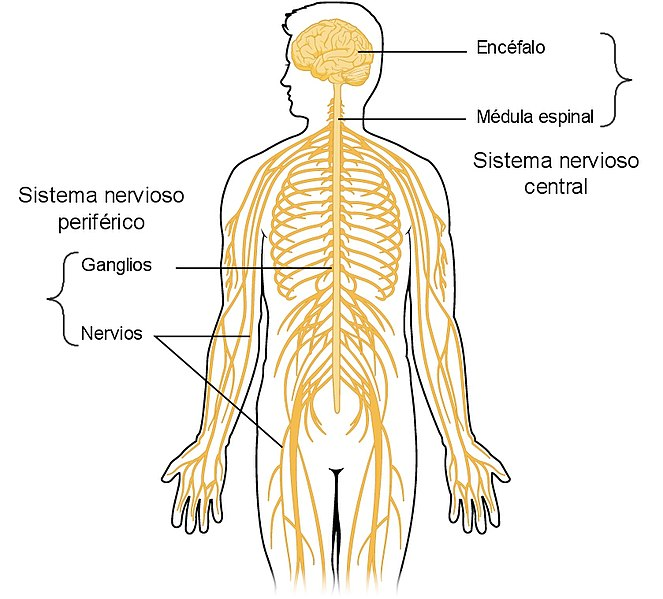
\includegraphics[scale=0.5]{../Figuras/Nervous_System.jpg}
 \caption{Overview of Nervous System esp, OpenStax, 20 December 2018, WIKIMEDIA COMMONS, \url{https://upload.wikimedia.org/wikipedia/commons/0/07/1201_Overview_of_Nervous_System_esp.jpg}, OpenStax, CC BY-SA 4.0}
 \label{fig:SNCySNP}
\end{figure}

En del sistema nervioso periférico tenemos al:

\begin{itemize}
 \item \textbf{Sistema somático} se controla de forma voluntaria, se conforma de nervios conectados a músculos voluntarios esqueléticos y receptores sensoriales, de los cuales unos son:
 \begin{itemize}
  \item de entrada, \textbf{aferentes}
  \item de salida, \textbf{eferentes}
 \end{itemize}

 \begin{figure}[h]
 \centering
 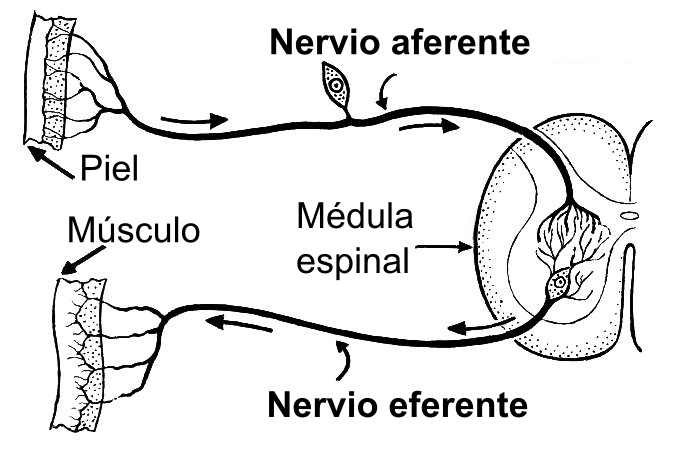
\includegraphics[scale=0.5]{../Figuras/afferent_efferent.png}
 \caption{Diagrama explicativo del recorrido eferente y el aferente, Pearson Scott Foresman, 26 August 2010, WIKIMEDIA COMMONS, \url{https://upload.wikimedia.org/wikipedia/commons/3/3e/Afferent_\%28PSF\%29.es.png}, CC0}
 \label{axonesSA}
 \end{figure} 
 
\item \textbf{Sistema autónomo} funciona de forma involuntaria, se conforma de nervios que se conectan con el corazón, los vasos sanguíneos, los pulmones, el estómago, los intestinos, glándulas
\end{itemize}

Ahora respecto al sistema nervioso central lo integra:

\begin{itemize}
 \item La médula espinal
    \begin{itemize}
     \item Dentro de esta hay una organización, la presencia de \textbf{ciclos de retroalimentación local}, es decir, nuestro sistema va a estar en diferentes etapas son nervios que no necesitan pasar por todo el procesamiento cerebral, las señales simplemente entran llegan a una fase local e inmediatamente reaccionan, ver el ejemplo de la imagen \ref{actReflejo}. Ocurren en un ciclo local y esto también puede convertirse en algo muy importante a la hora de hacer cómputos, no siempre es necesario pasar todo por todas las capas de procesamiento. 

     \begin{figure}[h]
      \centering
      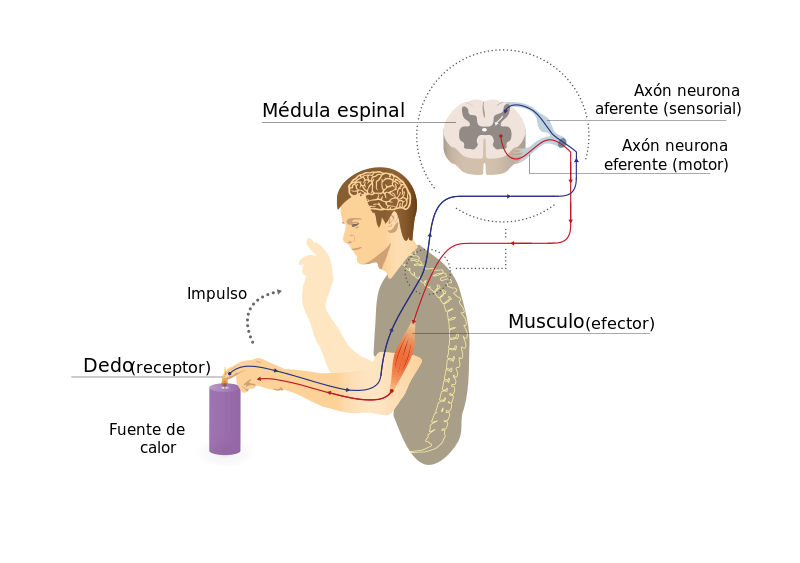
\includegraphics[scale=0.4]{../Figuras/actReflejo.png}
      \caption{ Esquema explicativo del arco reflejo, Marta Aguayo, 18 December 2014, WIKIMEDIA COMMONS, \url{https://upload.wikimedia.org/wikipedia/commons/c/cb/Imgnotraçat_arc_refelx_esp.svg}, CC BY-SA 3.0.}
      \label{actReflejo}
     \end{figure}

     \item \textbf{Señales de control motor descendientes} del cerebro hacia las neuronas motoras, estas son señales que provienen de un campo en una capa mucho más alta de procesamiento y provocan movimientos.
     
     \item \textbf{Axones sensoriales ascendentes} donde el cuerpo de la neurona está afuera y la información va a viajar hacia arriba, desde los músculos, piel y  estas señales viajan hasta el cerebro.  

     \end{itemize}

 \item El encéfalo
\end{itemize}

 Cada colección de nervios que sale de la base del cerebro se asocian con funciones muy específicas (en su mayoría). 
 
 Notas:
 
 \begin{itemize}
  \item Este sistema está hecho en diferentes niveles locales, entradas y salidas  
  \item El procesamiento que esté ocurriendo en el encéfalo puede tener diferentes capas y eso se verá reflejado cuando nosotros definamos arquitecturas para las redes neuronales. 
  \item Las redes neuronales actuales, que han tenido más éxito, se componen de diferentes subunidades o diferentes redes que hacen cosas locales. Es decir esta estructura global que estamos viendo,  se está empezando a reproducir/imitar ya con las neuronas computacionales.

 \end{itemize}


\subsection{Cerebro}

En esta parte vamos a preocuparnos sobre todo por la parte funcional. Haciendo una breve analogía, vamos a hacer una visión general del “hardware”, para ver qué efectos va a tener en el “software”. 
En general la arquitectura de cada cerebro es completamente diferente al cerebro de otras personas. Se ha intentado averiguar qué está haciendo cada región con diferentes estudios por ejemplo,  ver cuánta sangre se está bombeando en diferentes regiones del cerebro dependiendo de los estímulos que se le presentan a una persona, o si alguna persona tiene un padecimiento se tratan de tomar escaneos para ver qué regiones del cerebro están funcionando y cuáles presentan lesiones. A partir de las lesiones, lo que hacen es que una vez que está identificada la actividad que ya no se puede realizar de forma normal, averiguan qué región era responsable de esa actividad, que ahora está dañada.

Gracias a esos estudios, se ha logrado identificar más o menos en forma general, a qué se dedica cada una de las regiones del cerebro. En ocasiones no se puede decir exactamente qué tan vinculadas están (las regiones) o por qué se están activando otras regiones.

Hay partes funcionales que se comparten entre las diferentes regiones y no están ubicadas en un solo lugar. Otras parte importante a mencionar es, el cerebelo que se considera prácticamente vital, cumple con funciones tales como el equilibrio, la coordinación, el control fino de los músculos, de hecho tiene más neuronas que el cerebro y aún así hay niños que nacen y viven sin cerebelo. 


A continuación se mencionan algunas de las diferentes funciones de las regiones, que se han identificado en la imagen \ref{cerebro}: 

 \begin{figure}[h]
  \centering
  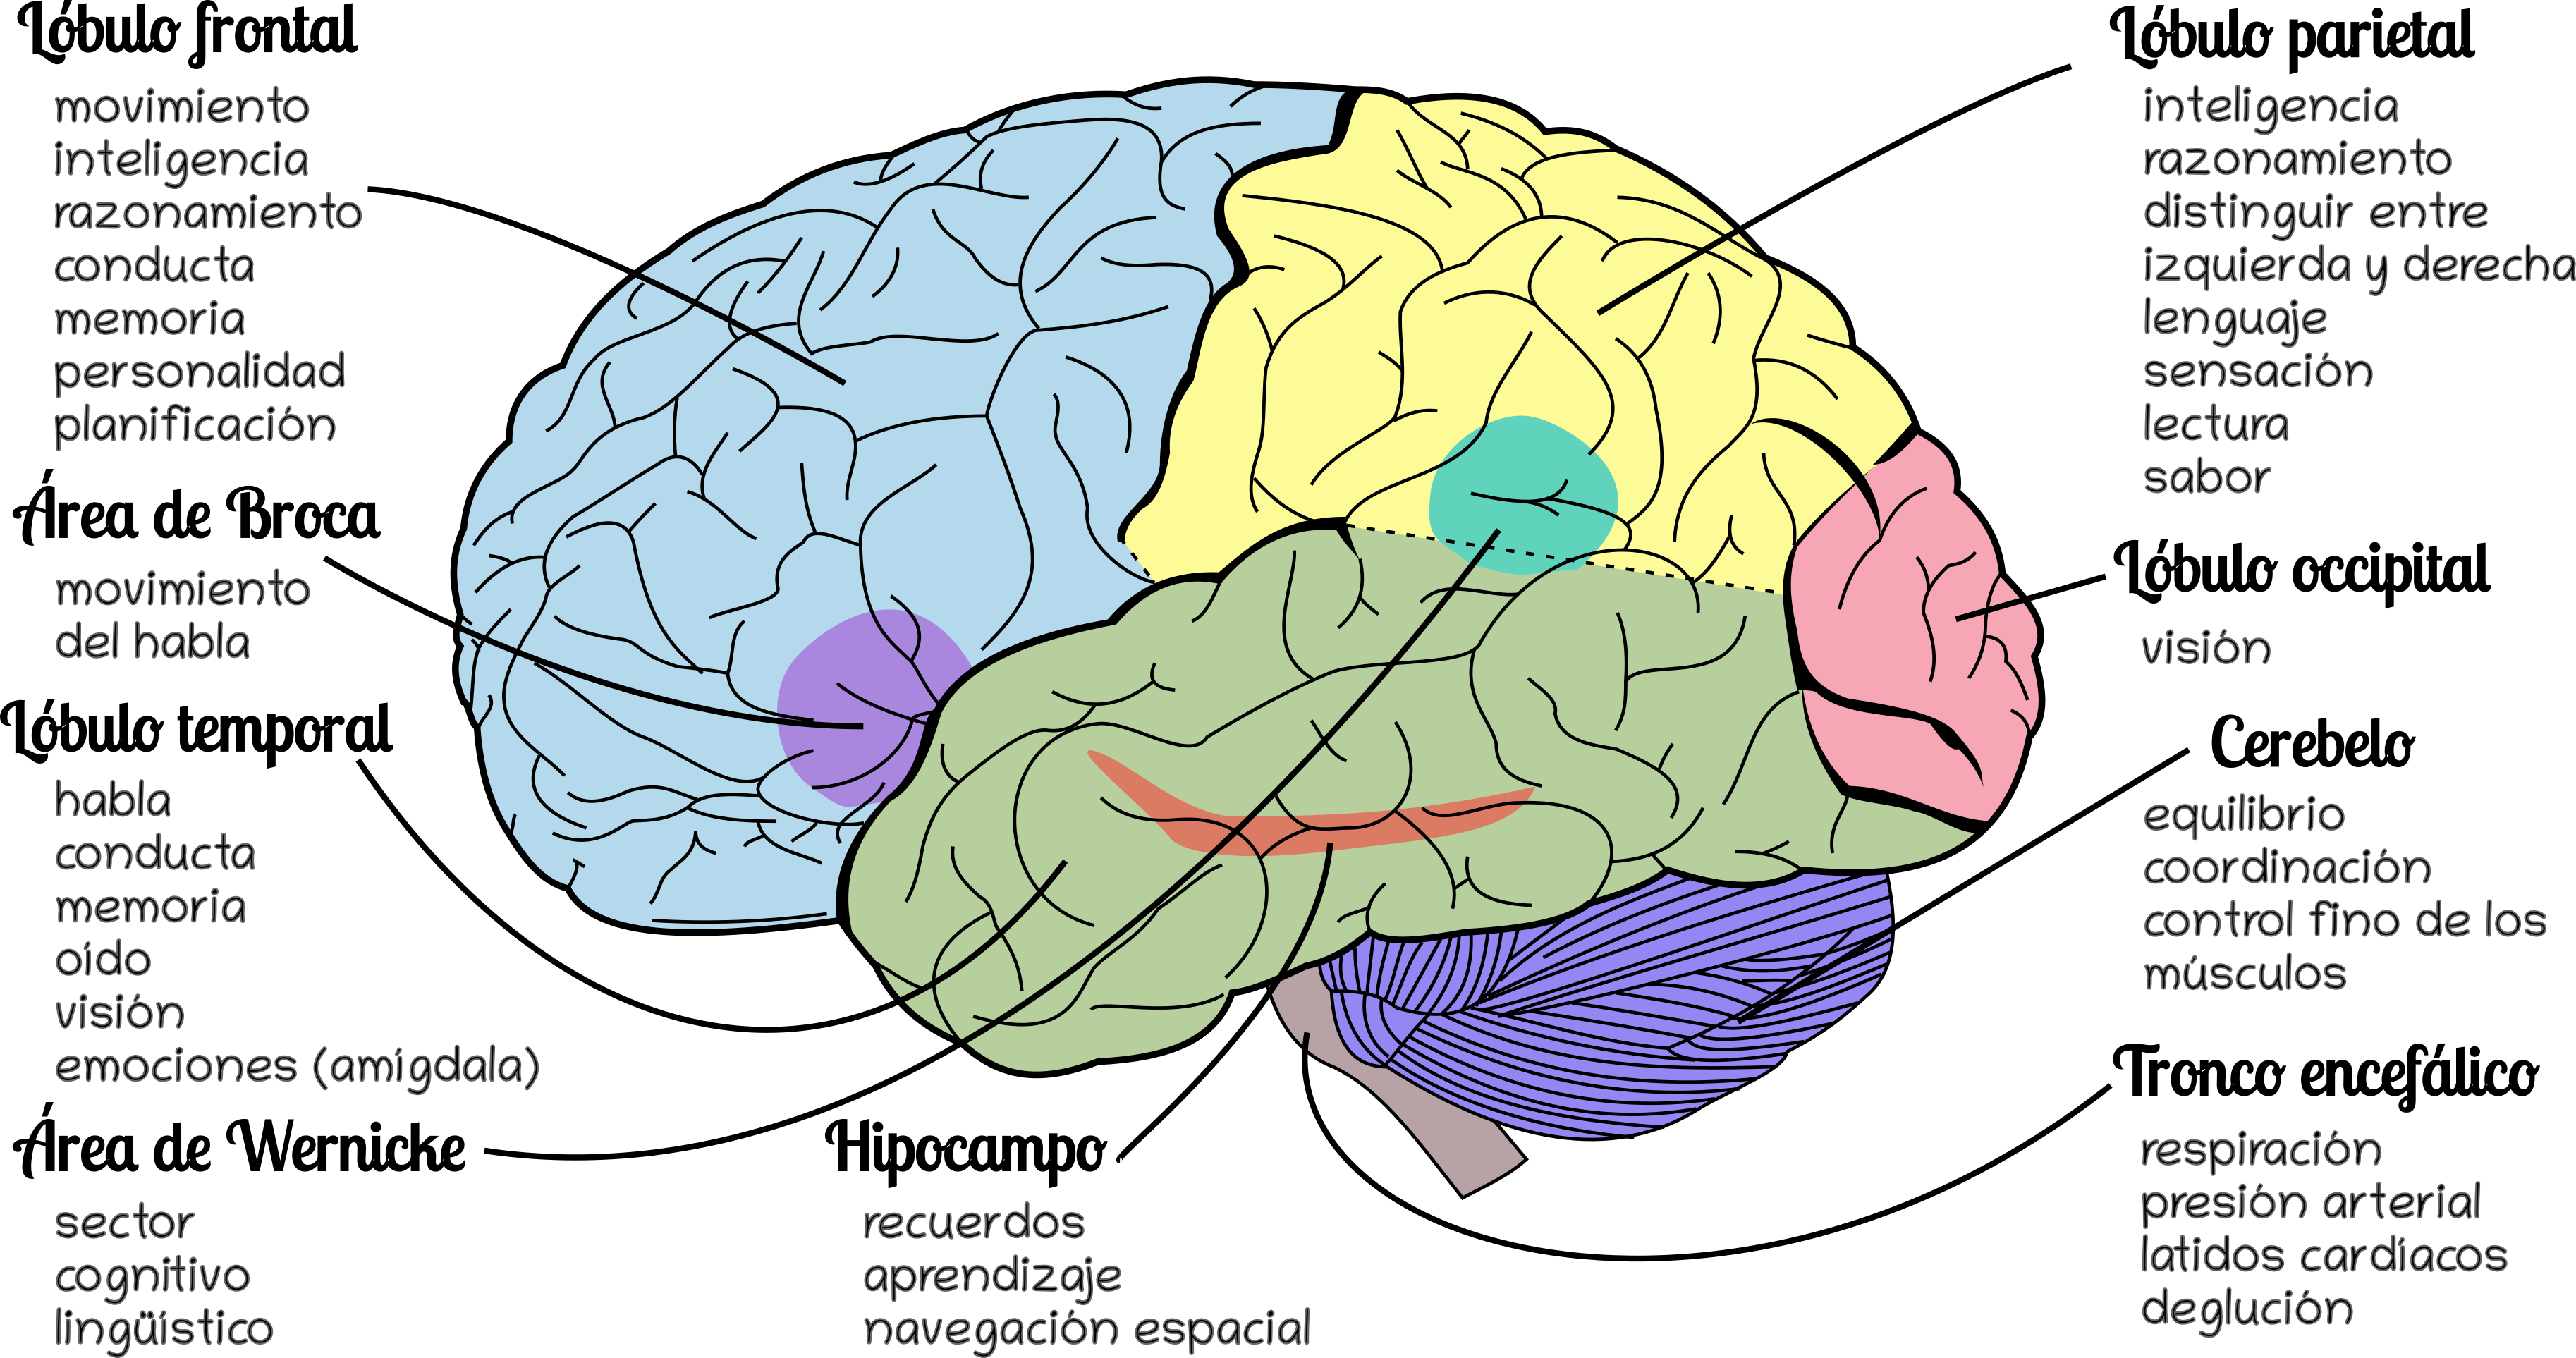
\includegraphics[scale=0.7]{../Figuras/cerebro.png}
  %Presentación Sistema Nervioso
  \caption{Diagrama básico de las regiones del cerebro.}\label{cerebro}
 \end{figure}

\begin{description}
%\begin{itemize}
 \item \textbf{Lóbulo frontal} se le puede asociar con la parte del raciocinio,  la parte de inteligencia, la conducta, la memoria, la personalidad, la capacidad para realizar planes complejos a largo plazo y también es responsable de algunas actividades de movimiento. Dentro de este destaca el área de broca, su principal función es el movimiento del habla, mover los labios, la boca.
 \item \textbf{Lóbulo temporal} aquí está otra parte del habla, que tiene que ver más con el uso de símbolos para el lenguaje, la conducta, memoria, aquí se procesa el oído, un poco de visión y emociones. Dentro de este está (compartida entre el lóbulo parietal) el área de Wernicke, trabaja con la parte lingüística, y de cognición. También dentro de este está el \textbf{hipocampo} trabaja con recuerdos, aprendizaje y navegación espacial, cómo sabemos cómo llegar de un lado hacia otro.
 \item \textbf{Lóbulo parietal} trabaja con la inteligencia, razonamiento, distinguir entre izquierda y derecha, lenguaje, sensación, lectura y sabor. 
 \item \textbf{Lóbulo occipital} se dedica prácticamente solamente a visión, es una región un tanto amplia. En particular en el área de robótica cuando están programando un robot o móvil, los robots tienen dos laptops y una de ellas se dedica prácticamente solo a procesar la visión.
 \item \textbf{Cerebelo} se encarga del equilibrio, la coordinación fina de los músculos.
 \item \textbf{Tronco encefálico} se encarga de la respiración, presión arterial, latidos cardíacos, de ilusión, conciencia. 
%\end{itemize}
\end{description}

\subsection{Zonas funcionales}
Para visualizar mejor la parte de la arquitectura, que tiene el cerebro para realizar todo lo que se le conoce como,  la ruta desde la sensación hasta la cognición, veremos un diagrama de la parte funcional del cerebro.  

 \begin{figure}[h]
  \centering
  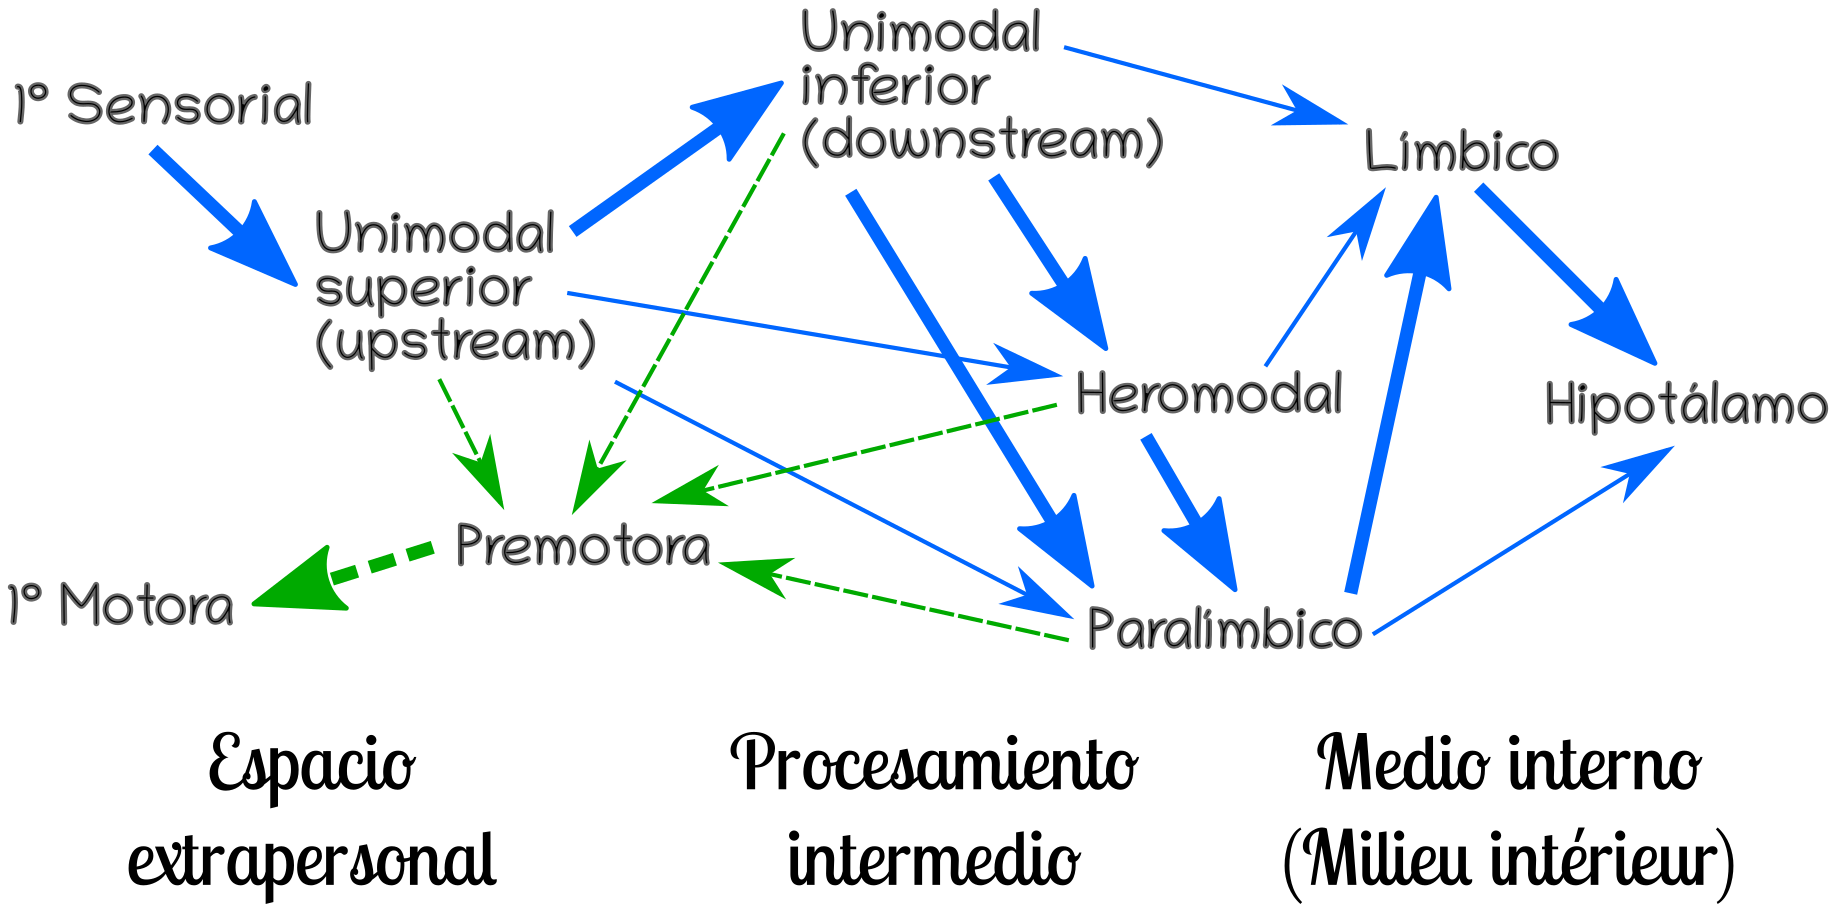
\includegraphics[scale=0.2]{../Figuras/zonasFuncionales.png}
  %Presentación Sistema Nervioso (11)
  \caption{Diagrama de la arquitectura del cerebro a nivel funcional.}
  \label{zonasFun}
 \end{figure}

Explicando el diagrama \ref{zonasFun}, en la primera parte (espacio extrapersonal) vamos a pensar en la entrada sensorial, que se enfoca muchísimo en la parte de visión y audio (en general todos los sentidos), notamos qué de las neuronas que están en la parte sensorial, su primera conexión es hacia una capa que se le llama unimodal superior,  aquí se procesa la información de cada sentido de manera individual, es decir, las neuronas o solamente están procesando visión o solamente audio, todavía no se mezclan, por ejemplo de visión, se separan colores e intensidad lumínica, se empieza a detectar algunas esquinas, alguna inclinación, la dirección de las luces y las sombras. Notemos que desde aquí hay una rápida conexión a la sección premotora y luego hacia la parte motora, recordando la mención de los circuitos locales y de reflejos, aquí prácticamente lo podemos ver (en este pequeño camino).

Pasando de este primer procesamiento básico entramos al siguiente que es el unimodal inferior, (aquí aún se está trabajando con procesamiento de una sola modalidad) visión sigue siendo visión, audio sigue siendo audio, pero ya son procesamientos un poco más complejos, por ejemplo, reconocimiento de rostros, de objetos. En esta parte tenemos un rápido ciclo de regreso a la parte premotora, por ejemplo la acción de ver a mi mamá y saludarla (aquí aún no se tiene que razonar demasiado). 

En la siguiente fase (medio interno), se conecta hacia tres áreas, la \textbf{heromodal}, ya se integran diferentes modalidades (audio y visión) ejemplo, oigo que me hablan y volteo a ver, aquí se está juntando ambas cosas, el \textbf{límbico} y el \textbf{paralímbico} que trabajan con la parte de las emociones y conceptos abstractos.

Finalmente llegamos al \textbf{hipotálamo} que es donde están todas las emociones, en las conexiones entre estas regiones, estarían los procesamientos de alto nivel.

Ahora estas diferentes regiones se replican de cierta manera cuando estamos haciendo los diseños de las arquitecturas modernas para redes neuronales.
En algunas ocasiones se comienza con algunas capas de neuronas, haciendo procesamientos con una sola modalidad, extrayendo datos básicos, después se van
componiendo en figuras más complejas y después hasta podemos combinar bloques de neuronas, para poder resolver problemas que tomen en cuenta diferentes modelos.




\section{Neurona biológica}
\subsection{La neurona}
La neurona es un tipo de célula perteneciente al sistema nervioso central, que se comunica tanto por señales eléctricas como por señales químicas. Cada neurona tiene:

 \begin{itemize}
	\item Un cuerpo celular (\textbf{soma}) que contiene un núcleo y otros componentes celulares.
	\item Una zona de recepción denominada \textbf{dendritas}.
	\item Una zona de emisión conocida como \textbf{axón}, compuesto de:
		\begin {itemize}
			\item Cono axonico.
			\item Membrana plasmática axonica y citoplasma.
			\item Recubrimientos de mielina, interrumpidos con intervalos regulares de nódulos (anillos) de Ranvier.
			\item Terminales del axón donde se encuentan los \textbf{botones sinapticos}. 
		\end{itemize}
 \end{itemize}

\begin{figure}[h]
 \centering
 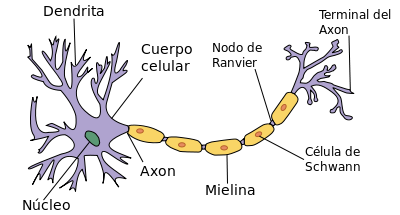
\includegraphics[scale=0.6]{../Figuras/neuronaPartes.png}
 \caption{Neurona, Acracia, 14 January 2007, Wikimedia Commons, \url{https://commons.wikimedia.org/wiki/File:Neurona.svg}, Creative Commons Attribution-ShareAlike 2.5 Generic}
 \label{fig:neuronaP}
\end{figure}

 Pensemos en la neurona como toda una compuerta, por un lado esta el cuerpo de una neurona típica, en las dendritas tenemos una mezcla de neurotransmisores y iones que pueden moverse a través de la membrana. La forma en que intercambia información es mediante sustancias químicas y iones que se están intercambiando, entre la parte de afuera y de adentro de la neurona. Particularmente en las dendritas, se tienen terminaciones que se pueden conectar con otras neuronas y de esta manera permitir el paso de información. 
 
 \begin{itemize}
  \item Neurona presinaptica, transmite una señal.
  \item Neurona postsinaptica, recibe una señal.
 \end{itemize}  
 
En el interior de la neurona hay una cierta carga eléctrica, en el exterior (el líquido de afuera) hay otra carga eléctrica, es decir, hay una \textbf{diferencia de potencial} entre el interior y el exterior de la neurona, por eso se dice que la membrana axónica en sí misma tiene una carga eléctrica. Dado que es porosa, esta membrana  va a estar intercambiando partículas con el exterior, esto va a hacer que la polarización de esta membrana vaya cambiando, si en algún momento la diferencia de potencial neta rebasa un cierto umbral.


\emph{Transmisón de señales y alacenamiento de información:}

\begin{enumerate}
 \item La neurona desde sus dendritas recibe señales de otras neuronas vecinas.
 \item Cada señal se va acumulando en su cuerpo hasta el cono axónico, donde se van a estar sumando la contribucion de todos los efectos de cambios de potencial.
 \item En el momento que se rebase un cierto valor umbral, la diferencia de potencial se propaga hasta los botones terminales.
 \item La neurona entra en un período refractario, donde empieza a cambiar el potencial entre el cono axónico y el axón de la neurona.
 \item Se va a transmitir un disparo eléctrico en seguida,
 \item La neurona se va quedar totalmente quieta, durante un breve momento para que la señal pueda viajar hacia el axón.
 \item Se va a notar un cambio muy violento en el voltaje, que se va recorriendo a lo largo de todo el axón. 
\end{enumerate}

La neurona tipica tiene unas células de mielina, que forman nodos que van cubriendo al axón para evitar que se pierda la señal, estos nodos recargan otra vez la señal y permite que avance, al siguiente nodo, donde se recarga  nuevamente y avance, hasta que logre llegar al final de axón.

\begin{figure}[h]
 \centering
 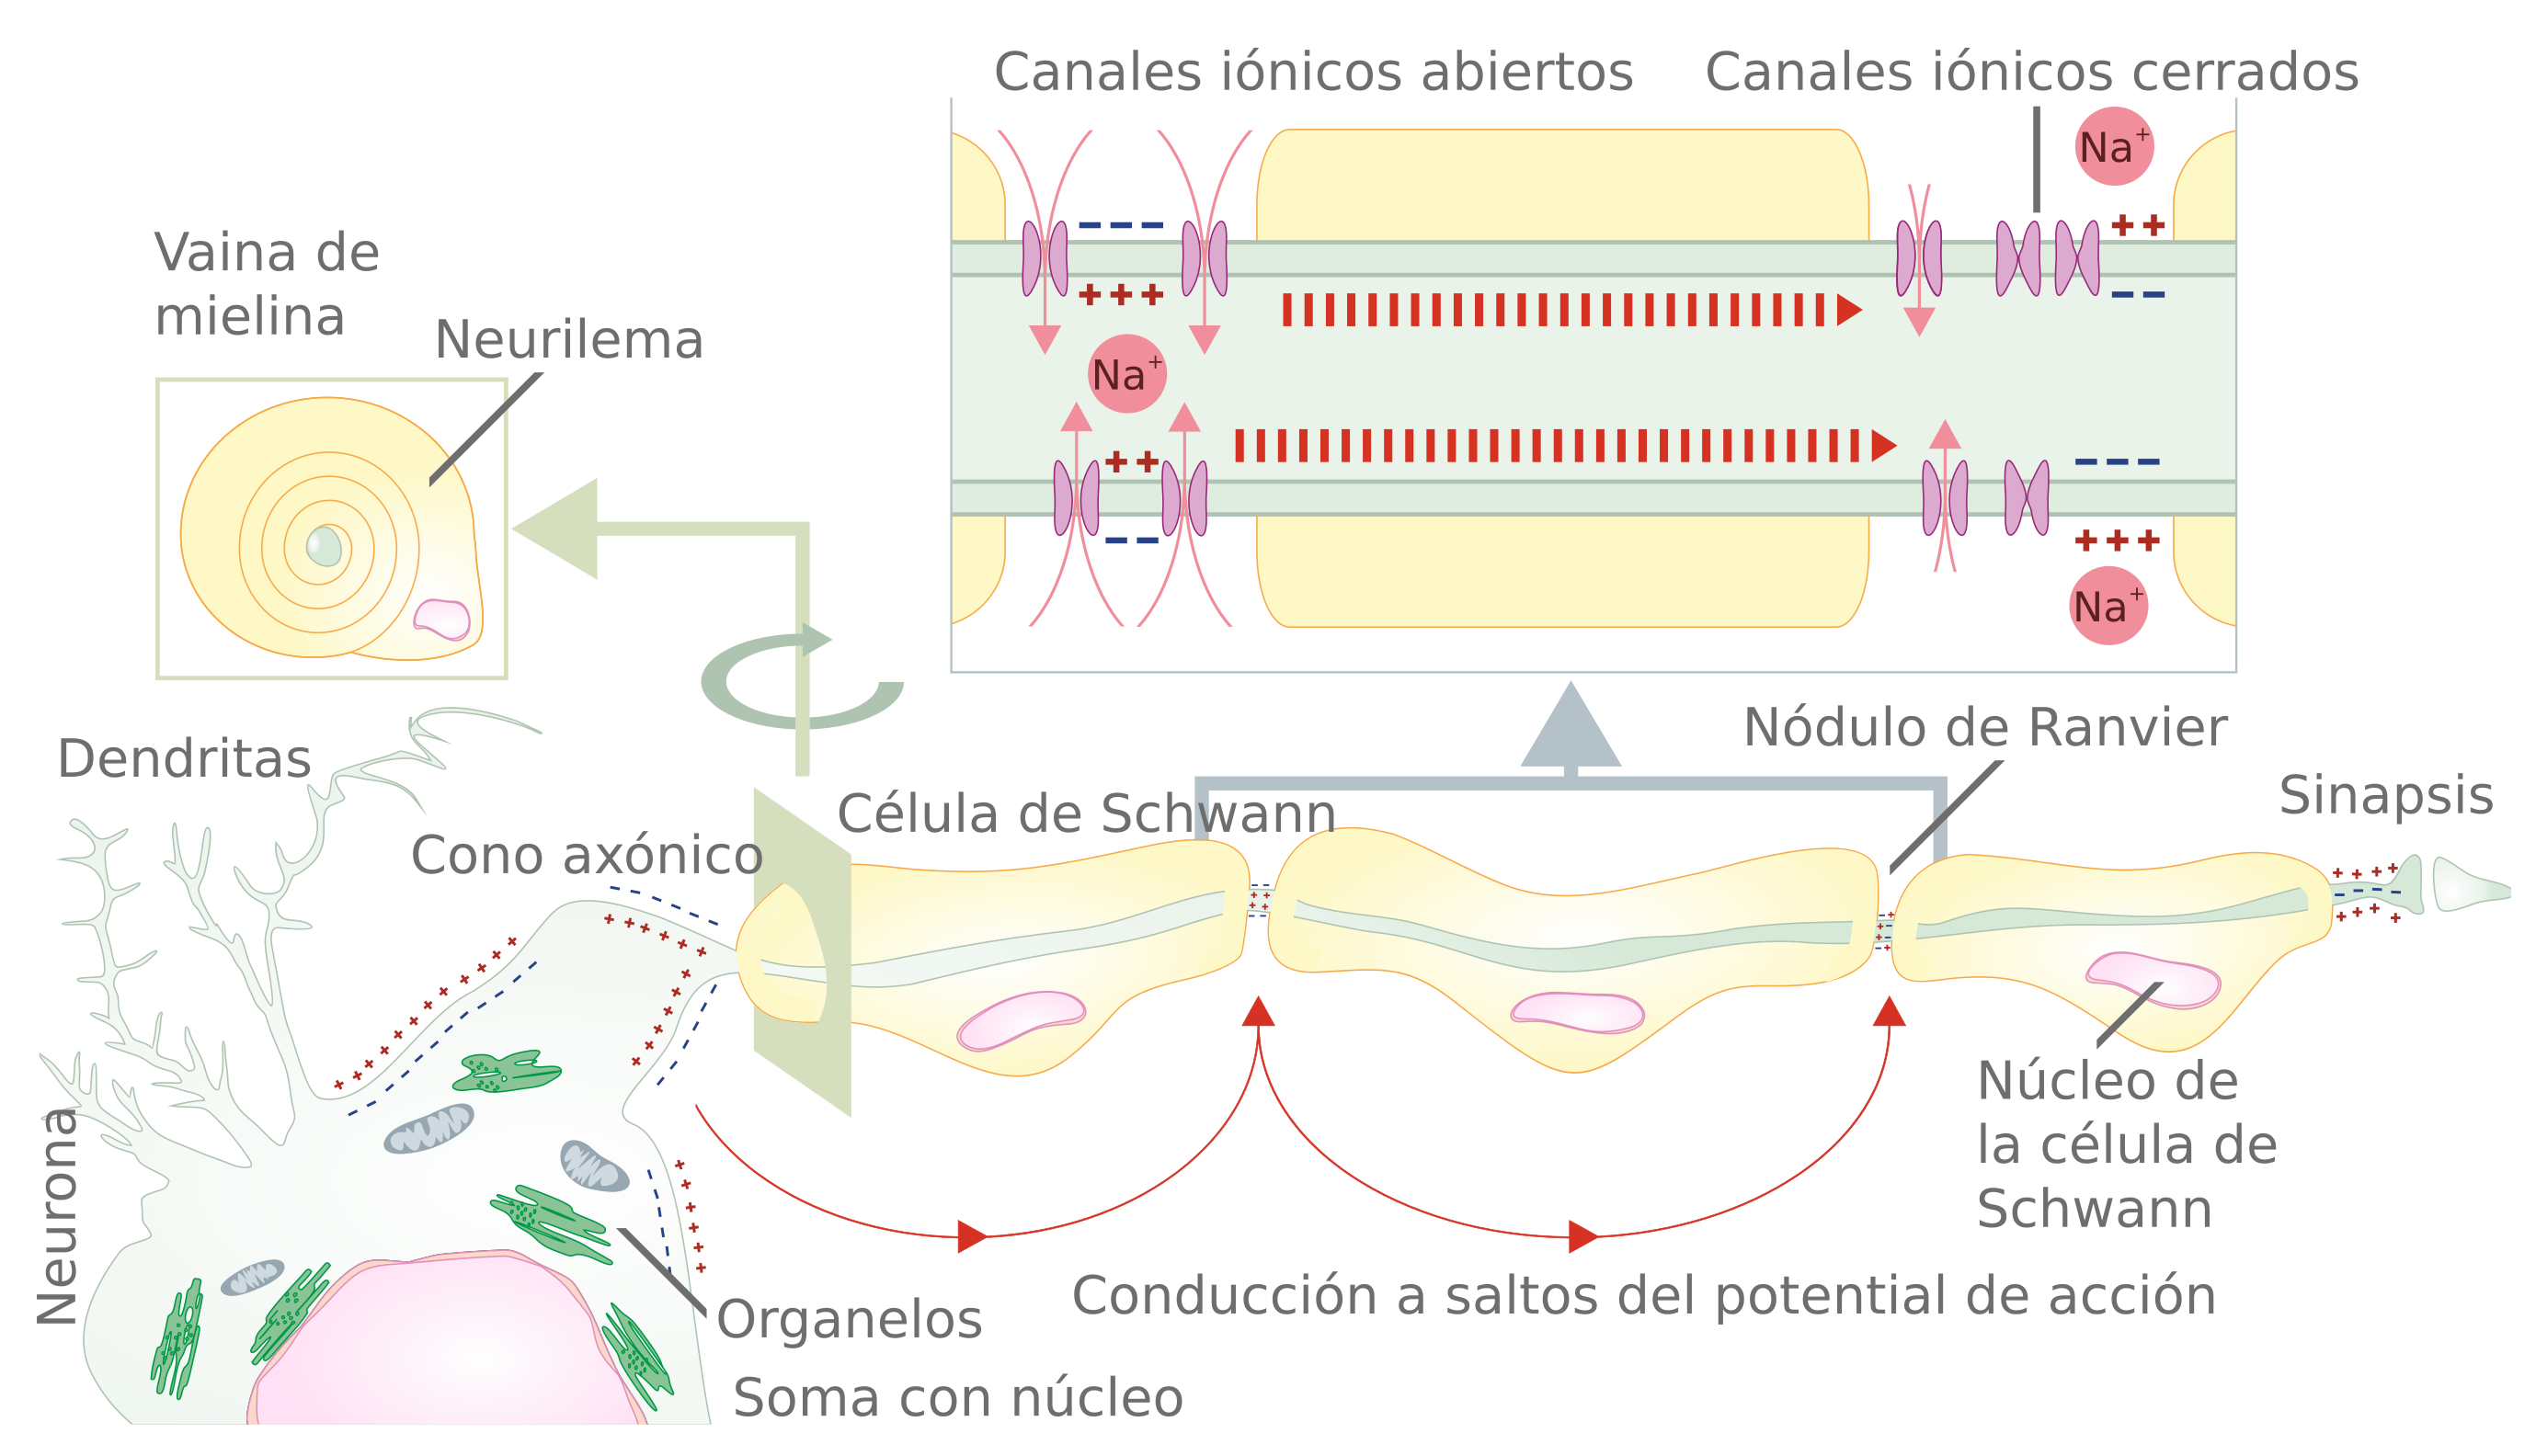
\includegraphics[scale=0.1]{../Figuras/Saltos.png}
 \caption{Corriente iónica por el axón (efecto de corto plazo), Helixitta, 1 October 2015, Wikimedia Commons, \url{https://commons.wikimedia.org/wiki/File:Propagation_of_action_potential_along_myelinated_nerve_fiber_en.svg}, Creative Commons Attribution-ShareAlike 4.0 International}
 \label{fig:conduccionSaltos}
\end{figure}

Este trayecto puede ser de una neurona a unas pocas neuronas vecinas, hasta unos cuantos metros (ej. esta podría estar en la médula espinal y el axón llegar hasta el dedo), Cuando la señal llega a la colita de la axón, hay varias terminales que van a reaccionar ante el cambio de electricidad, mediante la liberación de unas vesículas, que contienen \textbf{neurotransmisores}.


\subsection{Elementos de las neuronas y tipos}

Elementos durante la transmisión de señales:

\begin{itemize}
\item \textbf{Neurotransmisores:} son los mensajeros químicos que se comunican entre neuronas adyacentes; La liberación de neurotransmisores de una neurona ayudará a despolarizar o hiperpolarizar (aumentar la magnitud de la carga) la neurona adyacente, lo que hará que sea más o menos probable que ocurra un potencial de acción en la siguiente neurona.
  
\item \textbf{Impulsos eléctricos:} potenciales de acción que son, cambios de voltaje que van a ir ocurriendo a lo largo del axón. Sucede una vez que se acumularon demasiadas señales a través de las dendritas, entonces la neurona puede disparar un impulso eléctrico, a través del axón, que va a provocar que su terminal libere más químicos, estos químicos son los que hacen los efectos pequeños en cada uno de los cuerpos de las neuronas postsinapticas.
 
\item \textbf{Plasticidad:} modificación a largo plazo de las conexiones entre neuronas. En el cerebro las neuronas pueden cambiar de manera permanente, perder canales (que permiten el intercambio de nuevos transmisores sin impulsos eléctricos), formar más canales o incluso pueden crear protuberancias. Por ejemplo, cuando un cerebro aprende está transformando su arquitectura, es decir, los aprendizajes de largo plazo, modifican el cerebro y en consecuencia va a pensar y reaccionar distinto, que antes del aprendizaje.
\end{itemize}

\emph{Clasificación de tipos de neuronas:}


\begin{figure}[h]
 \centering
 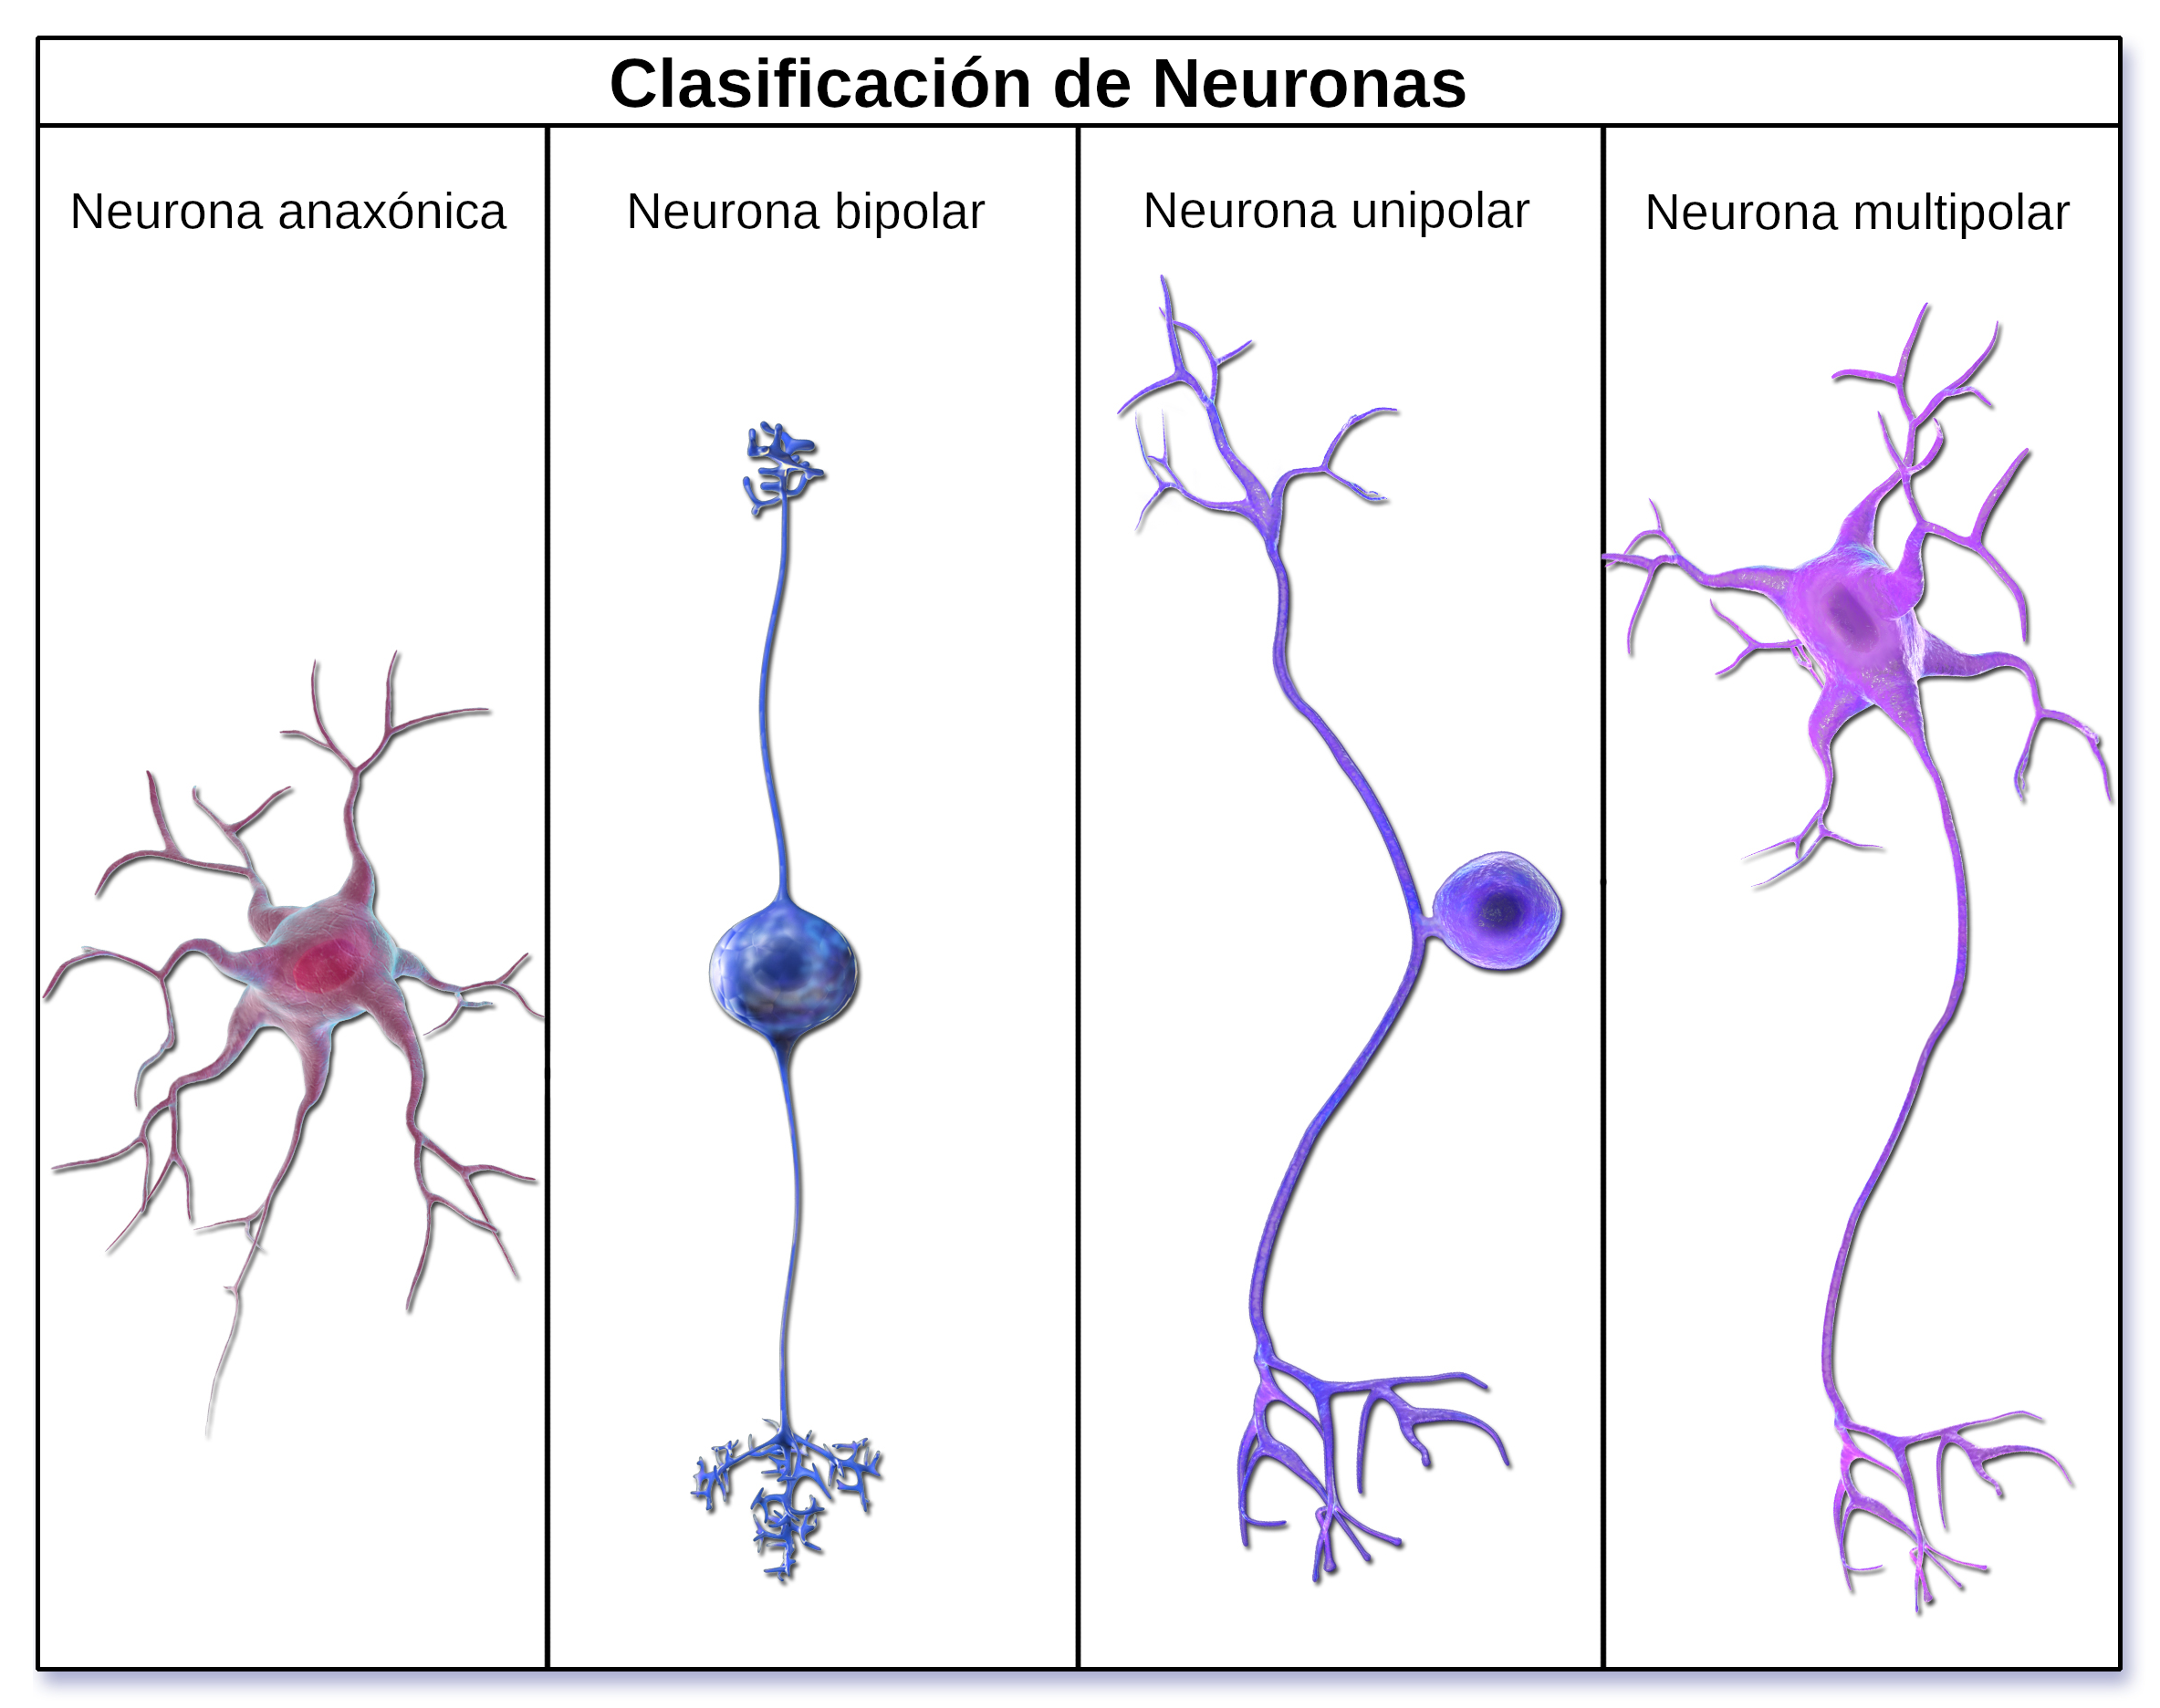
\includegraphics[scale=0.15]{../Figuras/tiposDeNeuronas.png}
 \caption{Representación de la clasificación de neuronas, BruceBlaus, 26 June 2017, Wikimedia Commons, \url{https://commons.wikimedia.org/wiki/File:Neuron_Classification.png}, Creative Commons Attribution-ShareAlike 4.0 International}
 \label{fig:tiposNeuro}
\end{figure}


\begin{itemize}
\item \textbf{Neuronas sin axones}, nunca dispara pero si tiene intercambios de neurotransmisores en las dendritas   
\item \textbf{Neuronas bipolares}, tienen dos axones. 
\item \textbf{Neurona unipolar}, solamente hay una conexión entre el cuerpo y el axón pero el axón tiene dos ramas, cuando dispare va a disparar hacia los dos lados, haciendo llegar su señal a diferentes regiones. 
\item \textbf{Neurona multipolar}, la más conocida, empieza con un cuerpo con dendritas y luego un largo axón que va a terminar con varias terminaciones axónicas. 
\end{itemize}

Cuando modelamos redes neuronales lo típico es modelar, una neurona con dendritas, su disparo y su axón, que se conecta con las siguientes dendritas, pero aquí ya estamos viendo que la naturaleza nos dice que hay que pensar más y plantear cómo hacer la representaciones de estas conexiones que nos presenta la naturaleza, un poco diferente pero tal vez con resultados más satisfactorios.


\subsection{Sinapsis}

Aquí veremos más a detalle cómo una neurona recibe o transmite información a otras neuronas, donde para un solo disparo están participando un montón de elementos que veremos más adelante.

 El momento en que dos neuronas transmiten información se llama \textbf{sinapsis} y es mediante conexiones que se dan en las terminales del axón (vesiculas sinápticas) de la neurona presináptica hacia la postsináptica. Es importante notar que estas neuronas no tienen contacto anátomico, sino que están separadas por un espacio muy pequeño, \textbf{la brecha sináptica}. Lo que sucede en estas conexiones es un intercambio electroquímico que produce cambios de polaridad a lo largo la membrana. 


\begin{figure}[h]
 \centering
 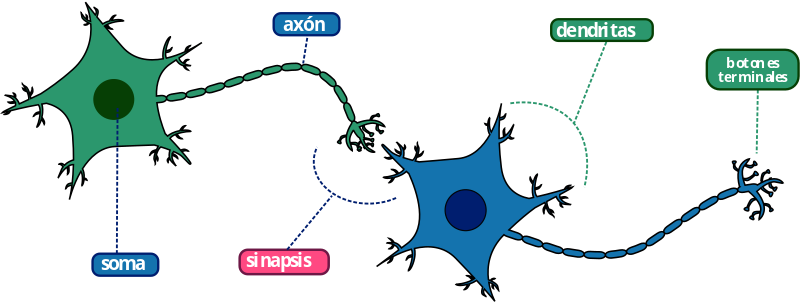
\includegraphics[scale=0.5]{../Figuras/Part_of_neurons_in_Spanish.png}
 \caption{Part of neurons in Spanish, Dana Scarinci Zabaleta, 24 February 2019, Wikimedia Commons, \url{https://commons.wikimedia.org/wiki/File:Part_of_neurons_in_Spanish.svg}, OpenStax, CC0}
 \label{fig:sinapsisN}
\end{figure}

Clasificación de sinapsis, las terminales del axón de la neurona presináptica puede hacer contacto con la neurona postsináptica en:
\begin{enumerate}
 \item su dendritas, axodendrítica.
 \item su cuerpo (soma), axosomática. 
 \item su axón, axoaxónica.
\end{enumerate}

Distingamos entre dos tipos de sinapsis:

 \textbf{Sinapsis eléctrica:} las membranas de las células pre y postsináticas se unen en la brecha sinaptica por una union tipo gap, o unión comunicante, que son pequeños canales que permitien el paso de iones.

	\begin{enumerate}
  	 \item Posee una transmisión bidireccional de los potenciales de acción.
  	 \item Sincronización en la actividad neuronal, lo cual hace posible una acción coordinada.
 	 \item Los potenciales de acción pasan a través del canal proteico directamente sin necesidad de la liberación de los neurotransmisores, por tanto es más rápida.
	\end{enumerate}

\begin{figure}[h]
 \centering
 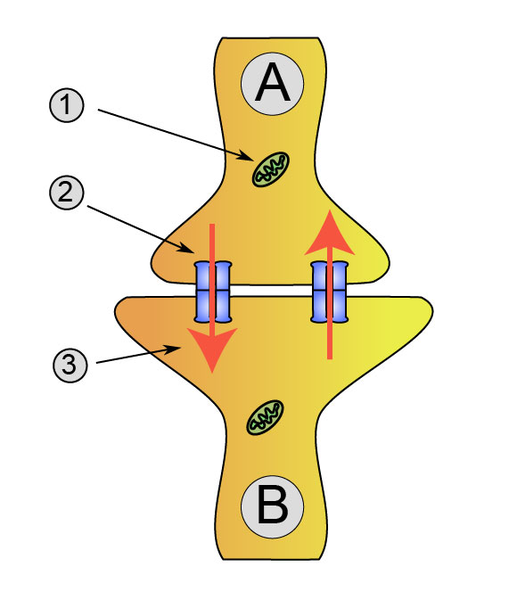
\includegraphics[scale=0.4]{../Figuras/sinapsisElectrica.png}
 \caption{Synaptical transmission (electrical). Neurona A transmisora, Neurona B receptora, 1. mitocondria, 2. uniones gap formadas por conexinas, 3. señal eléctrica , Nrets~commonswiki, 23 September 2005, Wikimedia Commons, \url{https://commons.wikimedia.org/wiki/File:Synapse_diag2.png}, Inkscape 0.42, CC-BY-SA 3.0}
 \label{fig:sinapsisN}
\end{figure}
 
 \textbf{Sinapsis química:} la neurona libera moléculas neurotransmisoras a otra neurona adyacente en un pequeño espacio (la brecha sináptica) ver \ref{fig:sinapsisQ}. Se puede resumir en cuatro etapas principales:

\begin{enumerate}
 \item Un potencial de acción llega al boton terminal proviniente desde cono axónico.
 \item Los neurotransmisores contenidos en las vesículas que están el los botones terminales, son liberados en la brecha sináptica y se dispersan.
 \item Cada neurotransmisor se une a su receptor ubicado en la membrana de la neurona postsináptica.
 \item El exceso de neurotransmisores que queda en el espacio sináptico es degradado o recaptado.
\end{enumerate}

\begin{figure}[h]
 \centering
 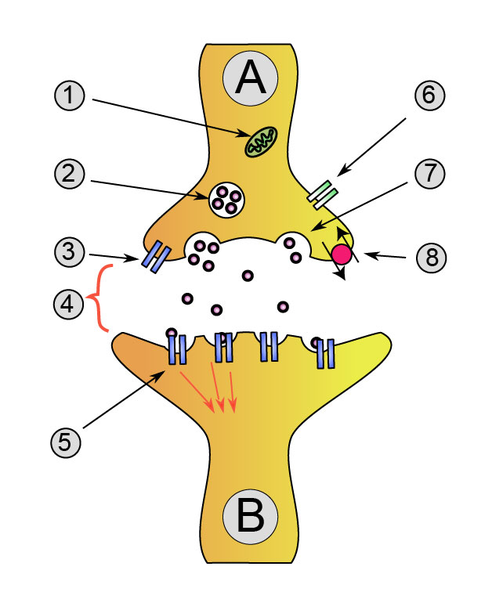
\includegraphics[scale=0.4]{../Figuras/SinapsisQuimica1.png}
 \caption{Synaptical transmission (chemical). Neurona A transmisora, Neurona B receptora, 1. mitocondria, 2. vesícula sináptica llena de neurotransmisor, 3. autorreceptor, 4. brecha sináptica, 5. receptor de neurotransmisores, 6. canal de calcio, 7. neurotransmisor liberador de vesículas fusionadas, 8. bomba de recaptación de neurotransmisores, Utilisateur:Dake, 23 September 2005, Wikimedia Commons, \url{https://commons.wikimedia.org/wiki/File:Synapse_diag1.png}, Inkscape 0.42, CC-BY-SA 3.0}
 \label{fig:sinapsisQ}
\end{figure}


Detallando el procesos de la sinapsis química, la neurona postsináptica está recibiendo un montón de señales por la liberación de neurotransmisores tanto de sus vecinos, como lo que ella misma va intercambiando, una vez que están generando el efecto completo de cambiar la polarización de la membrana, van a provocar que la neurona haga un disparo eléctrico. En el cuerpo están llegando estos intercambios de iones que se suman en el cono axónico, empiezan a viajar a través del axón, en las vainas de mielina (donde se refuerza la señal). 
Aquí hacemos mención por primera vez de los iones positivos: sodio y potasio, estos iones lo que hacen es, que \emph{la membrana tenga una cierta carga la mayor parte del tiempo}. Cuando salen tres sodios entran dos potasios, entonces siempre hay más positivos afuera que en el interior de la neurona, es decir, por lo general  \emph{tiene una carga más negativa que su entorno} (ver \ref{fig:MembranaP}). Cuando ocurre un disparo de la neurona y se da el cambio de polarización en la membrana, se abren sus poros/ canales. El hecho que los canales abran o cierren depende de varios cambios que puedan estar ocurriendo alrededor de la neurona, en particular los que transmiten el disparo eléctrico, reaccionan ante el cambio de potencial que ocurrió en la membrana de la neurona. 

La señal va pasando por los nodos de Rainvier, se refuerza y pasa por los canales iónicos ya abiertos, hasta finalmente llegar a la sinapsis a esto le llaman la \textbf{conducción a saltos} (ver \ref{fig:conduccionSaltos}). Ahora lo que ocurre al final del recorrido es que, el cambio de electricidad otra vez provoca que unas vesículas, que están en el interior de la neurona, que contienen neurotransmisores, se peguen a la membrana axónica y se liberen esos neurotransmisores nuevamente a otra neurona. 

Entonces la información le va a llegar a la neurona vecina, en la forma de neurotransmisores que fueron liberados (en lo que sea que lo haya recibido, típicamente son dendritas, pero podría ser su cuerpo o su axón), eso es lo que va a percibir la otra neurona y otra vez esta otra neurona va a empezar a sumar los efectos de estos neurotransmisores, para que en algún momento decida a lo mejor disparar y otra vez provocar que se liberen neurotransmisores a su final e influir con otras neuronas.

\subsubsection{Neurotransmisón}
Cuando la neurona no está mandando señales eléctricas, tiene un potencial de reposo, su diferencia de potencial entre el interior y el exterior de la neurona, es más negativo en el interior y más positivo (o menos negativo) en el exterior.
En el caso de las sinapsis químicas, llega un disparo y se altera el potencial de la membrana, entraran las
células de calcio y entra la participación de las vesículas para liberar neurotransmisores. Los neurotranmisores estan flotando en la brecha sináptica, viajan hasta adherise a los receptores de la neurona postsinaptica, en ese momento están alterando el intercambio normal que existe entre \underline{iones en el interior y en el exterior} de la célula y van a cambiar las cargas netas que hay adentro y afuera. Este es un cambio local que está ocurriendo en una puntita de una dendrita, 

\begin{figure}[h]
 \centering
 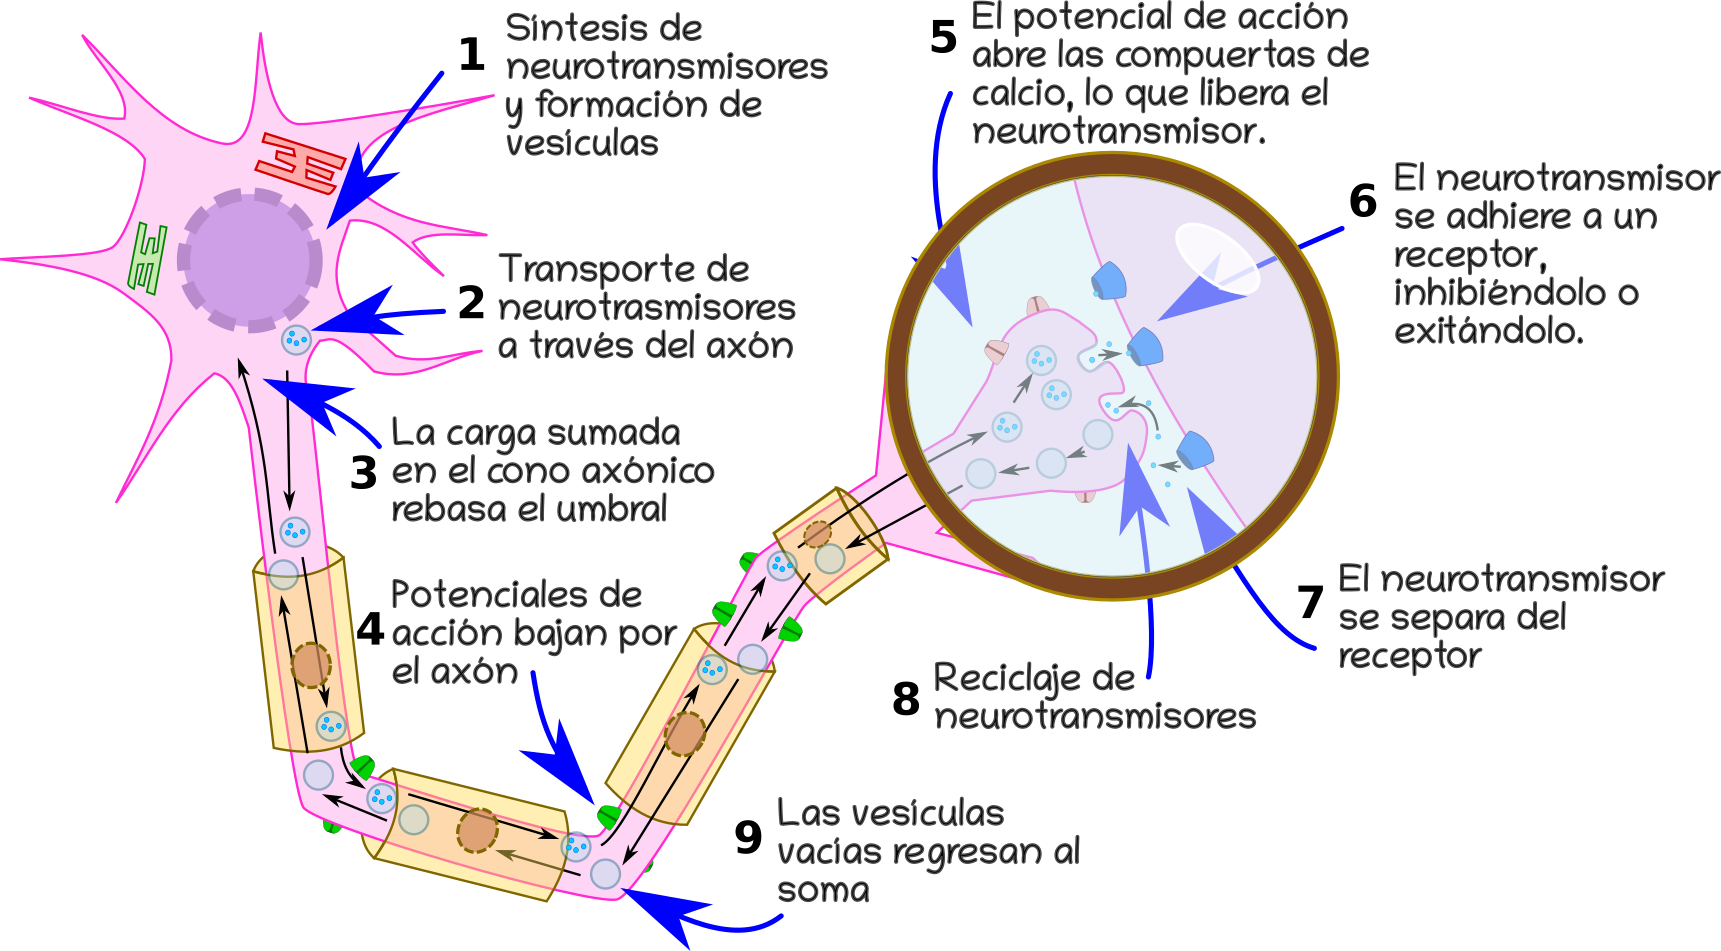
\includegraphics[scale=0.2]{../Figuras/neurotransmision.png} 
 \caption{Esquema detallado de una neurotransmisión.}
 \label{fig:nTransmision}
\end{figure}

este cambio en sí es una especie de transferencia de información pero muy local, entonces podemos distiguir entre dos efectos en la membrana: 

\begin{itemize}
\item \textbf{El efecto excitatorio}, despolariza la membrana postsináptica es decir ahora va a ser más propensa a disparar porque ya le cambió la diferencia de potencial que tenía.  
\item \textbf{El efecto inhibitorio}, hiperpolariza la membrana postsináptica, es decir, va a incrementar la diferencia de potencial entre el exterior e interior pero de tal manera que ahora ya no va a querer disparar esta neurona.
\end{itemize}

De estos efectos también va a darse el efecto de la \textbf{plasticidad}, que es cuando dos neuronas tienden a excitarse juntas, después de esta conexión se va a tender fortalecer, sí más bien tienden a inhibirse lo que va a suceder después es que estos canales empiezan a encoger, haciendo que se reduzcan y ya no dispare.

Ejemplos de neurotransmisores: serotonina, dopamina, oxitocina, endorfinas, adrenalina.


\subsection{Campos receptivos}
Aquí lo que nos interesa es, en qué región puede ser afectada una neurona. Se define un campo receptivo, como la región en la periferia sensorial
dentro de la cual los estímulos pueden, influir la actividad de las células sensoriales (ver \ref{fig:camposR}). Hay diferentes niveles donde pueden aparecer los campos receptivos tanto cerca de la piel, cerca del gusto, el olfato, donde las neuronas van a estar asociadas con otras células que les pueden ayudar, que son sensitivas a los cambios correspondientes, a veces la misma neurona va a tener alguna protuberancia especializada.
También podemos encontrarlos más hacia adentro del nivel de procesamiento, no necesariamente todos van a estar pegados a la parte sensorial física. 
\begin{figure}[h]
 \centering
 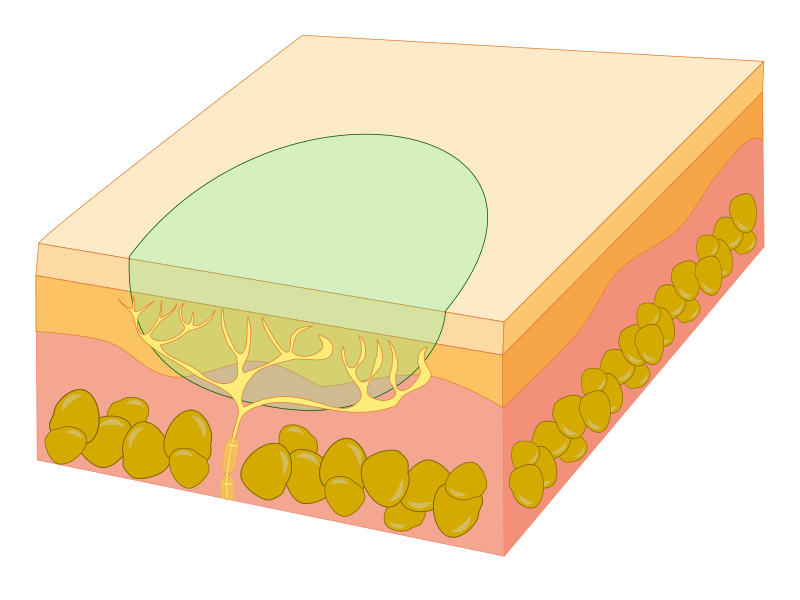
\includegraphics[scale=0.3]{../Figuras/camposreceptores.png}
 \caption{Campo receptivo. Se muestra una región que está bajo cierto estímulo, las terminales de la neurona está recibiendo está información y transmitiendola.}
 \label{fig:camposR}
\end{figure}

Comprenden a los receptores sensoriales que alimentan a las neuronas sensoriales, pueden ser:

\begin{itemize}
\item Receptores específicos en una neurona como protuberancias especializadas. 
\item Conjuntos de receptores capaces de activar una neurona mediante conexiones sinápticas. 
\item Describen la ubicación donde debe estar presente un estímulo sensorial para licitar una respuesta desde una célula sensorial. 
\end{itemize}

Ejemplos:

\begin{itemize}
\item En la piel tenemos células que nos están protegiendo en la epidermis, una de las células auxiliares \textbf{la célula de merkel} que es
sensible a la presión. Esta puede estar muy cerca a una neurona, sus terminales se activan de acuerdo a las acciones de la célula de Merkel y va a pasar la información (ver \ref{fig:mer}).  
 	
\begin{figure}[h]
 \centering
 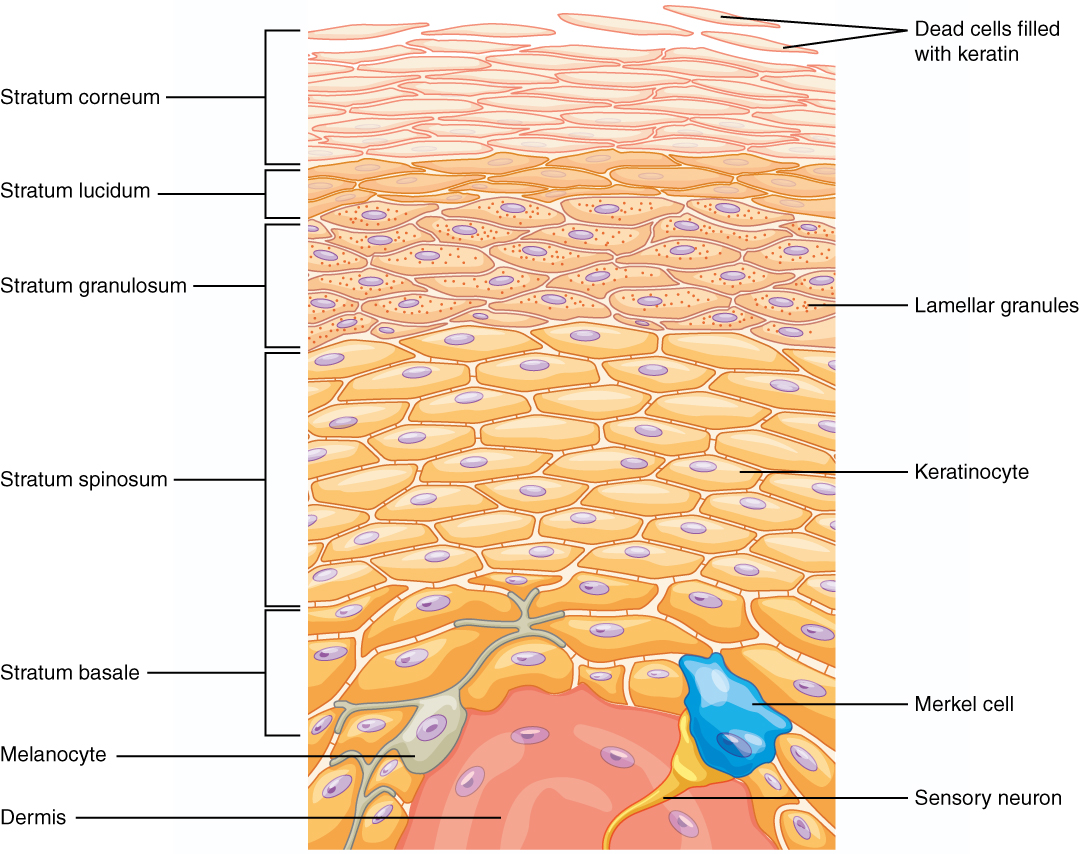
\includegraphics[scale=0.2]{../Figuras/merkel.png}
 \caption{Capas de la epidermis y en azul la célula de Merkel.}
 \label{fig:mer}
\end{figure}

\item El ojo, para procesamiento visual, actualmente se utiliza una de las redes neuronales más famosas que son las redes convolucionales, que están inspiradas en el ojo, nosotros tenemos campos receptores donde hay unos fotorreceptores en los conos y los bastones que son sensibles a luces de diferentes colores a cambios de intensidad de la luz y que pueden detectar, por ejemplo, en una cierta región física si está llegando luz  o por ejemplo, si llega en la periferia entonces va a inhibir el disparo de estos elementos, por otro lado tenemos también su complemento que permite ser estimulado por las señales que llegan, como que en la parte de afuera de un círculo y más bien se inhiben con un estímulo en la parte de afuera (ver \ref{fig:nSen}). Esta especie de celdas que tienen una posición física y geométrica relevante van a determinar cuando disparan o no las neuronas. Los siguientes niveles del cerebro se van a encargar de interpretar mejor  el cambio de sombras, como a una persona que pasó corriendo, un auto que se está moviendo cerca o reconocer algún tipo de alimento.
\end{itemize}

\begin{figure}[h]
 \centering
 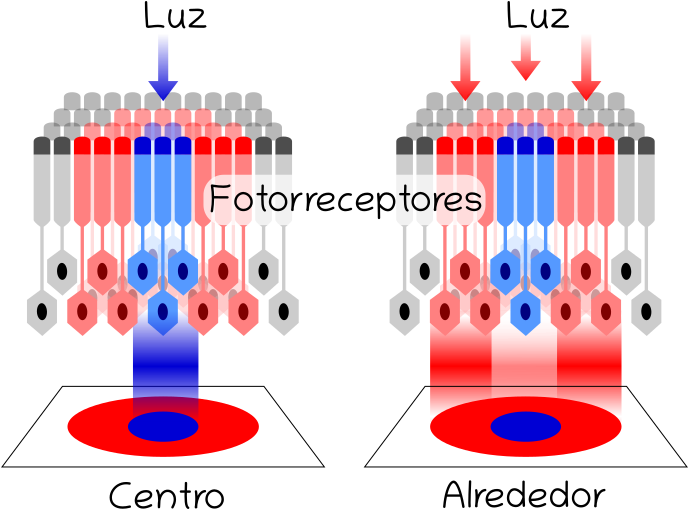
\includegraphics[scale=0.5]{../Figuras/nSensitivas.png}
 \caption{Capas de la epidermis y en azul la célula de Merkel.}
 \label{fig:nSen}
\end{figure}


\subsection{Señal eléctrica}
Veamos que pasa en los canales de iones y el paso de la señal eléctrica primero diferenciemos los tipos de compuertas iónicas:

\begin{itemize}
\item \textbf{Canal por fuga:} Estos se abren y cierran aleatoriamente, todo el tiempo están activos en la neurona, intercambiando por ejemplo: sodio y potasio.
\item \textbf{Canal regulado por ligado:} Aquí se hace presente un neurotransmisor que es el que va a provocar que se abran o al revés impedir que se abran.
\item  \textbf{Canal por estímulo mecánico:} Permiten que pasen más iones o menos iones dependiendo, si se ejerció una presión, por ejemplo, con las neuronas cerca
de la piel, las células de merkel.
\item \textbf{Canales regulados por el voltaje:} Tienen el rol protagónico en la transmisión del pulso eléctrico (que se ha estado mencionando) describiendo uno de ellos, este canal tiene una pequeña compuerta abajo, que la puede cerrar independientemente del hecho de que el canal se abre o se cierre. Existen varias variantes de este tipo de canales regulados por el voltaje, la forma en que se están activando y desactivando sus compuertas, es lo que permite el paso del pulso.
\end{itemize}

Existen realmente una buena cantidad de iones presentes en el cerebro pero los más protagónicos son precisamente el \textbf{potasio}, el \textbf{sodio}, el \textbf{cloro} y son los que vamos a utilizar para un modelo matemático de las neuronas. 

\begin{figure}[h]
 \centering
 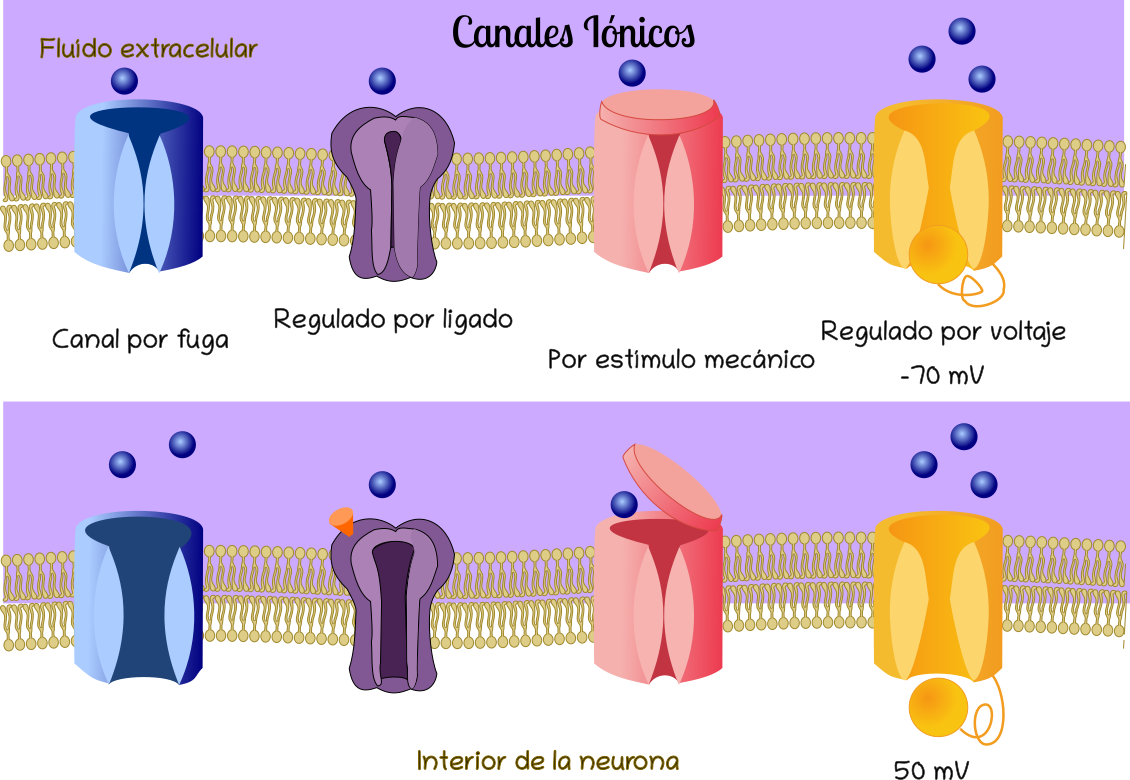
\includegraphics[scale=0.28]{../Figuras/canalesIonicos.png}
 \caption{Representación de la clasificación de los canales iónicos (más representativos).}
 \label{fig:MembranaP}
\end{figure}


Por ultimo veamos brevemente \textbf{la neuroplasticidad}, es lo que nos permite el aprendizaje a largo plazo en el cerebro, es un mecanismo de aprendizaje del cerebro en el cual:

Cuando las neuronas se activan simultáneamente con frecuencia la conexión entre ellas se fortalece.

Este mecanismo constituye la principal inspiración para el diseño de las redes neuronales artificiales, concretamente en esto se inspiran los algoritmos de entrenamiento. Lo que se hace es calcular, qué conexiones debemos reforzar y cuáles debemos de debilitar para que nuestras redes neuronales calculen las funciones que a nosotros nos interesan.

\begin{figure}[h]
 \centering
 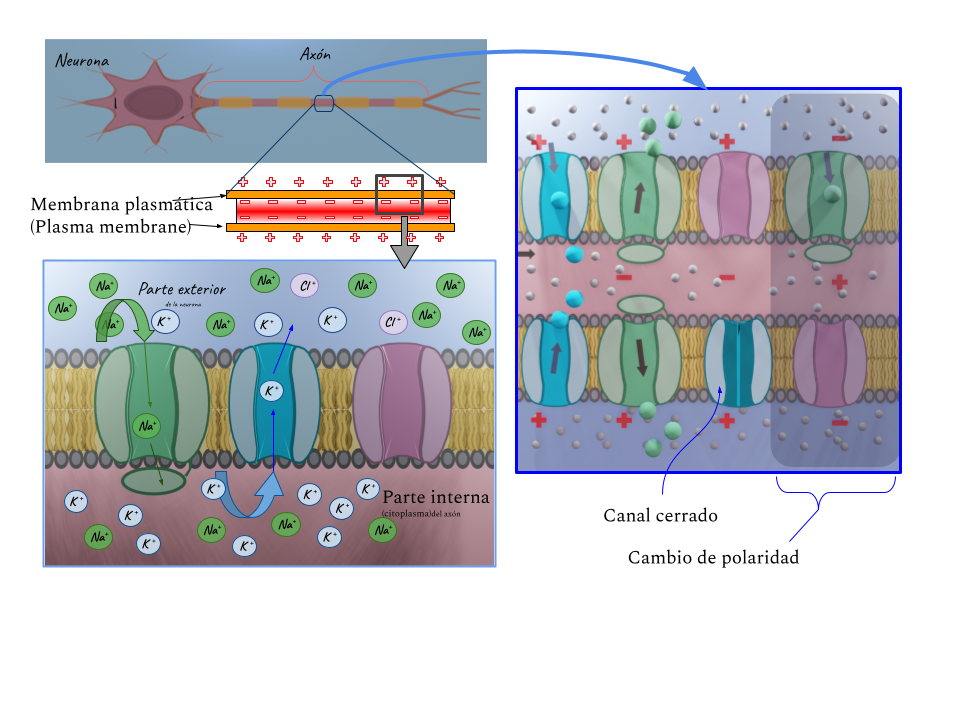
\includegraphics[scale=0.5]{../Figuras/MembranaP.png}
 \caption{Representación de la membrana axónica en potencial de reposo en la parte infererior izquierda, y el la parte derecha con un estímulo que genera el cambio de polaridad en la misma, así como el cierre de canales y paso de iones.}
 \label{fig:MembranaP}
\end{figure}




\chapter{Modelo de Hodgkin-Huxley}

\section{Introducción}
Esta sección se enfocará a la parte de transmisión de información y que tipo de operaciones lógicas matemáticas ocurren para que un cerebro pueda realizar cómputos, específicamente se detallará la mecánica de los disparos de las neuronas, siendo estos una de las características más relevantes a la hora de modelar las redes neuronales artificiales. Si en algún momento de su vida han visto temas relacionados con compuertas digitales, arquitectura de computadoras, diseño electrónico digital, les será más fácil abstraer el concepto, pues nosotros vamos a ver los procesos de paso de información a través de compuertas pero en un sistema biológico (de la naturaleza). 

Notemos primeramente un impulso nervioso, recordemos que esté es una onda que avanza desde el cono axónico de la neurona hasta la neurona postsináptica. Esta onda electroquímica ocurre dada la diferencia de potencial entre la parte interna y externa de neurona, está diferencia se da a consecuencia de las distintas concentraciones de iones en ambos lados de la membrana plasmática. Los estados en la membrana plasmática (del axón) se pueden diferenciar en, potenciales neuronales:

\begin{itemize}
\item \textbf{Potencial de reposo:} Es la diferencia de cargas en la membrana y está polarizada a -70mV. Es positiva por fuera (Na+ ) y negativa por dentro por Cl- y proteínas- y no transmite señal. 
\item \textbf{Potencial de acción o membrana:} Un estímulo umbral de 55mV, despolariza la membrana y abre los canales del Na+ y K+ y avanza la señal nerviosa, es un cambio muy rápido en la polaridad de la membrana de negativo a positivo y vuelta a negativo.
\end{itemize}

%(Insertar esquema) 
\begin{figure}[h]
 \centering
 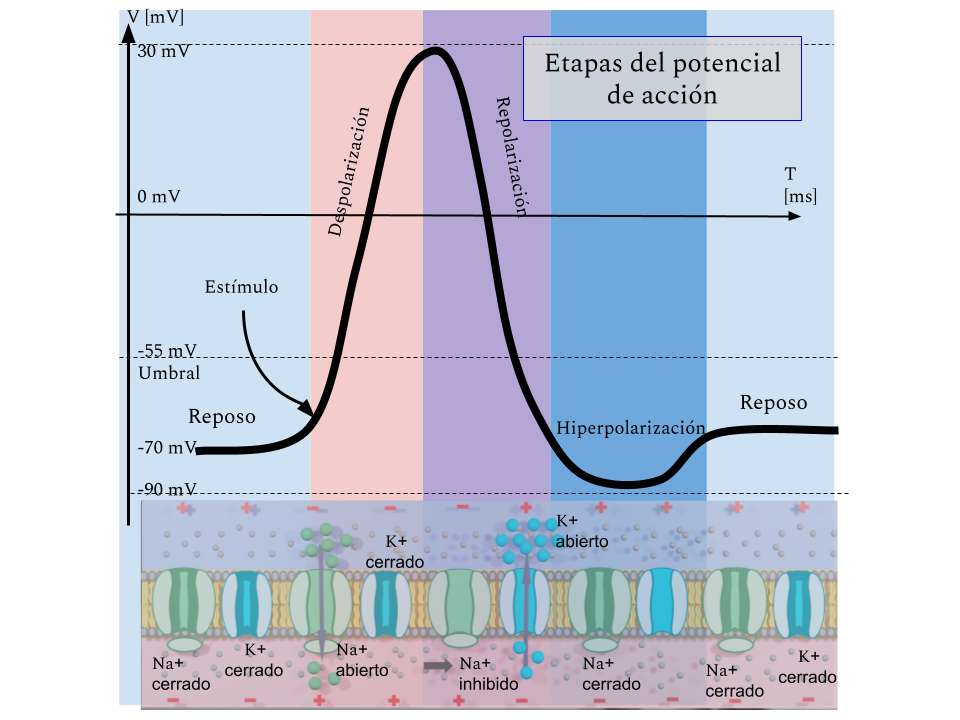
\includegraphics[scale=0.5]{../Figuras/Grafica.png}
 \caption{Representación gráfica de la respuesta de los canales ionicos de sódio (Na+ en verde) y potasio (K+ en azul) ante un estímulo de voltaje, dando como resultado un potencial de acción que viajará a lo largo de todo el axón.}
 \label{fig:graficaP}
\end{figure}

Retomando la sinapsis eléctrica, donde participan los canales iónicos y las entradas de la neuronas (dendritas) están siendo alteradas poco a poco, hasta que ocurre la suficiente carga (diferencia de potencial) en sus dendritas y en el cuerpo de la neurona, para que desde el cono axónico se de un disparo o potencial de acción (spike), transmitiendo la información gracias a la apertura y cierre de ciertos canales de iones cargados. Este cambio brusco de la diferencia de potencial, se nota en forma de un pulso eléctrico (ver \ref{fig:graficaP}),  para saber más a detalle qué está ocurriendo en está rápida elevación en la diferencia de potencial, se contará de dónde salió este modelo y por qué toma la forma que tiene. 

Los primeros científicos que estudiaron el potencial de acción y dieron un modelo (de la unión sináptica eléctrica) fueron Alan Lloyd Hodgkin y Andrew Fielding Huxley alrededor de 1952, obteniendo un modelo matemático \footnote{El texto original de este experimento se puede encontrar en la siguiente url: \url{ https://physoc.onlinelibrary.wiley.com/doi/pdf/10.1113/jphysiol.1952.sp004764}}, que intenta explicar qué es lo que estaba pasando en las neuronas. Ellos trabajaron con un calamar gigante (que puede medir hasta 4 metros de largo) que dado su gran tamaño, tiene un axón también bastante gigantesco, que recorre casi la mitad del cuerpo del calamar y su grosor es de medio milímetro, considerando el tamaño estándar de una axón de una neurona (1-20 µm). El axón del calamar gigante es tan grande que les permitió introducir dispositivos para medir el voltaje, es decir, la diferencia de potencial entre, el interior de la neurona y la parte de afuera (el ambiente externo de la neurona). Con estás mediciones experimentales que lograron obtener, se pudo determinar qué pasaba con las cargas eléctricas tanto en el interior como en el exterior y así estudiar cómo se lograba la transferencia de electricidad cuando disparaba este pulso. 
 Se dan cuenta que podían modelar este comportamiento como un circuito eléctrico donde están corriendo estas corrientes, si bien aún no sabían todavía cuál era exactamente el mecanismo biológico por detrás, si observaron que había dos elementos protagónicos que serían el sodio y el potasio.
 Notaron que estos existen en diferentes concentraciones, en la parte de afuera y en la parte de adentro de las neuronas. Con esto nosotros podemos aprender también el por qué es importante consumir algo de sal y nunca estar bajos de potasio, pues estos dos elementos son indispensables para que las neuronas puedan transmitir sus señales. 

\section{Membrana y canal}

Hodgkin y Huxley se dedicaron a estudiar qué pasaba con las concentraciones de estos iones (sodio y potasio) en la parte de afuera o en la parte de adentro cuando empezaban a fluir las corrientes. El sistema parecía una especie de circuito eléctrico, se lo imaginaron como una especie de membrana porosa (lo cual es bastante cercano a lo que después se descubrió  con la microscopía) y la forma en que lo vieron fue como un circuito eléctrico donde  \textit{la membrana está funcionando como un capacitor} que almacena ligeramente las cargas cuando están tratando de pasar de un lado hacia el otro y además con la cualidad que tenía de veces dejar pasar más iones y a veces no (semipermeable), modelan esto como una especie de \textit{resistencias variables}. Bajo ciertas condiciones de voltaje de la diferencia de potencial entre la parte de afuera y la parte de adentro, estos canales permiten pasar más de estos iones (ya sean sodio, potasio o calcio) o por el contrario impiden su paso (ver \ref{fig:ModelHh}).


\begin{figure}[h]
 \centering
 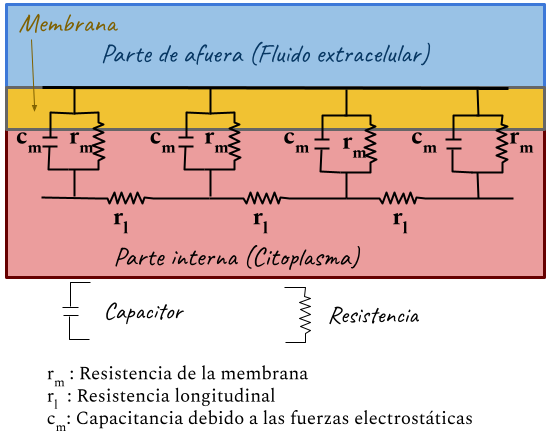
\includegraphics[scale=0.5]{../Figuras/ModeloHH.2}
 \caption{Un primer modelo de la membrana axónica modelada como circuito eléctrico. La parte amarilla es la membrana}
 \label{fig:ModelHh}
\end{figure}


Ahora se necesitan más detalles de la representación de los canales y toman en cuenta que el comportamiento de estas resistencias viene acompañado con un voltaje de reposo, en estos voltajes particulares cada tipo de ion (de la resistencia modelada) se estabiliza y ya no va a cambiar esta resistencia (ver \ref{fig:circuito}). 


\begin{figure}[h]
 \centering
 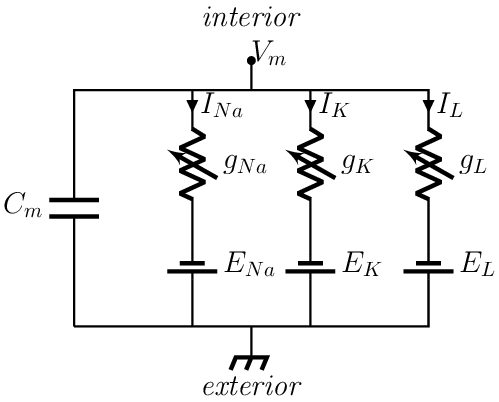
\includegraphics[scale=0.5]{../Figuras/circuito.png}
 \caption{Modelo de la membrana axónica modelada como circuito eléctrico, con los distintos canales presentes y su voltaje de reposo.}
 \label{fig:circuito}
\end{figure}

Lo que observan es que el \textbf{ion de sodio (Na+)} y su resistencia va a variar dependiendo del voltaje, a esto se le llama un \textbf{canal transitorio} porque en ciertos voltajes si puede pasar; si es muy bajo, no puede pasar y si rebasa un cierto umbral entonces se vuelve a tapar y ya no puede pasar. 
Lo que sucede con el \textbf{ion de potasio (K+)} es que, puede salir si el voltaje está más allá de un cierto valor, si no, no pasan y va variando un poquito que tanto puede pasar, a esto se le llama \textbf{canal persistente}. Por estas características de que el potasio es un intervalo dentro de la recta y el sodio es a partir de cierto valor, por tanto se les modelan de maneras ligeramente diferentes. Más adelante se descubrió porque tenían este comportamiento, básicamente el canal de potasio es una puerta hecha de cuatro subpuertas por donde los elementos pasan o no pasan, el canal de sodio es como una compuerta que está hecha de tres subpuertas que se pueden abrir y tiene aparte un tapón extra, que hace que  aunque estas tres están abiertas bloquee toda la compuerta.
Las neuronas están trabajando con muchos más iones aparte de estos dos, uno que destaca bastante es el caso del cloro (Cl-) que tiene carga negativa. Se tienen canales para intercambio aleatorio de otros iones, \textbf{L} un canal aleatorio (leaky).

Entonces con lo que ellos midieron experimentalmente, midieron cómo se estaban comportando estas resistencias dependiendo del voltaje o la diferencia de potencial que había entre ambos lados de la membrana y a partir de ahí pudieron describir matemáticamente y simular los disparos que se conocen como potenciales de acción vamos a ver cuáles fueron estos conceptos de electricidad que se están utilizando para el modelo tenemos este concepto de potenciales eléctricos.

\begin{itemize}
\item Potenciales eléctricos \emph{E ó  V}; resultan de la separación de cargas opuestas. Se mide en \emph{mV}.
    \begin{itemize}
     \item \emph{E\textsubscript{(Na,K,L)}} voltaje en reposo para los iones de Na, K y L, o también conocido como  potencial de inversión iónico, es el potencial de membrana en el que no hay flujo neto (total) de ese ion en particular de un lado de la membrana al otro. 
     \item \emph{V\textsubscript{m}}, el potencial eléctrico de la membrana. 
     \end{itemize}

\item Corriente \emph{I}; Movimiento de cargas. Se mide en \emph{µA}.
    \begin{itemize}
     \item \emph{I\textsubscript{(Na,K,L)}} corriente entrante a los canales de Na, K o L.
     \end{itemize}

\item Resistencia \emph{R}; Medida de la oposición al movimiento de las partículas cargadas.
\item Capacitancia o capacidad eléctrica \emph{C} . Cantidad de energía eléctrica almacenada en un capacitor para una diferencia de potencial eléctrico dada.
    \begin{itemize}
     \item \emph{C\textsubscript{m}} la capacitancia de la membrana. 
     \end{itemize}

\item Conductancia \emph{g}; Inverso de la resistencia \( \dfrac{1}{R} \) , es decir, facilidad de transmisión de las partículas cargadas.
    \begin{itemize}
     \item \emph{g\textsubscript{(Na,K,L}}  la conductancia del canal de sodio, potasio, cloro y la L también refiriendose a otros canales de iones. 
     \end{itemize}

\end{itemize}

Lo que está pasando en los \textbf{potenciales eléctricos} es que hay mucho sodio en la parte externa de la membrana por ej. tres iones de sodio que son cargas positiva por dos iones de potasio que hay en la parte interna, entonces hay muchas más cargas positivas en la parte de afuera que las que hay en la parte de adentro y eso es lo que provoca  la diferencia de cargas que es lo que estamos viendo como un  potencial eléctrico.

La  capacidad eléctrica o \textbf{capacitancia} es la que estamos utilizando para modelar la membrana conformada por lípidos, que es una  capa de grasa y esa es la cantidad de energía eléctrica almacenada en un capacitor para una diferencia de potencial eléctrico dada.Éste comportamiento bastante interesante porque las cargas quedan almacenadas un momento pero se van liberando poco a poco y se va descargando ese capacitor. 

Durante el experimento con el axón, se le dierón cargas electricas directamente al axón y gracias a eso lograban ir midiendo que era lo que estaba pasando con las concentraciones de cargas afuera y adentro en el caso de las neuronas reales, esto en un ambiente no alterado ocurre cuando entran en juego los neurotransmisores y provocan que haya cambios, en estas corrientes. Entonces hodgkin y huxley  jugaron el rol que tendrían que jugar usualmente los \emph{neurotransmisores} para abrir otras compuertas. Nosotros en la manera en la que lo vamos a simular es precisamente con estas corrientes que son las que se están poniendo en el experimento y vamos a ver cómo reacciona el axón. 


\section{Potenciales de Nerst o de reposo}

Son los potenciales a los cuales el flujo neto de iones a través de los canales abiertos es cero.
Aquí vemos precisamente porque estamos utilizando la \emph{E} generalmente la vamos a utilizar para referirnos a la diferencia de potencial entre la parte de afuera de la célula y la parte de adentro  las vamos a utilizar para representar a aquellos voltajes donde cada una de las compuertas encontrarían su equilibrio . Esos voltajes son distintos para cada una de las compuertas, esto va a provocar precisamente la dinámica de la de la neurona, por ejemplo: 

\begin{itemize}
\item E \textsubscript{Na}  \emph{50mV}
\item E \textsubscript{Ca}  \emph{150mV}
\item E \textsubscript{K}   \emph{− 80mV}
\item E \textsubscript{Cl}  \emph{− 60mV}
\end{itemize}

Aquí vemos que el sodio estaría su equilibrio en un valor positivo, 
el calcio que es el que va a jugar un rol de que se activen los neurotransmisores y se transmita el disparo, observamos que el voltaje tendría que ser bastante positivo. El potasio que es el que usualmente está trabajando intercambiándose casi todo el tiempo en la neurona, veremos que el punto de equilibrio usual de la neurona anda por los -76mV y el del cloro, cada uno de estos canales pues está tratando de jalar la dinámica hacia su potencial de equilibrio y no hay precisamente un acuerdo entre ellos y eso es precisamente lo que hace que las neuronas cobren "vida".

\section{Modelo de la membrana como bicapa de lípidos}
\hypertarget{LaEq}{La membrana} de una neurona es modelada como un elemento de un circuito con capacitancia \emph{C\textsubscript{m}} y potencial \emph{V} ,las corriente que fluye a través de la bicapa lipída están regidos por las siguientes ecuaciones:

\begin{equation}
  I_{m} = C_{m} \dfrac{dV_{m}}{dt}
  \label{eq:corrientesEnLaMembrana}
\end{equation}

Está sería la ecuación principal (\ref{eq:corrientesEnLaMembrana}) donde \(\dfrac{dVm}{dt}\) está representando el cambio voltaje en la membrana respecto al tiempo.

\begin{equation}
  C_{m} \dfrac{dV_{m}}{dt} =  - g_{Na} m^3 h(V - E_{Na} ) - g_{K} n 4 (V - E_{K} ) - g_{L} (V - E_{L} ) + I_ext
  \label{eq:corrientesEnLaMembrana2}
\end{equation}

Cada una de las partes del lado izquierdo de la ecuación \ref{eq:corrientesEnLaMembrana2} corresponde a las compuertas de los canales y la corriente de un estimulo externo que pueda influir a la membrana (este estimulo siempre será desde al exterior hacia el interior).

Retomando lo escrito anteriormente el canal de sodio es una compuerta compuesta de \textbf{tres} subpuertas y una subpuerta que actua como tapón y el canal de potasio es una compuerta compuesta de \textbf{cuatro} subpuertas iguales, \hypertarget{secc} {con esto podemos notar claramente que las conductancias sean representadas como}:

\begin{itemize}
 \item \(\dfrac{1}{R_{Na}} = g_{Na} * m ^3 * h \) donde \(g_{Na}\) es una constante que representa el valor de la conductancia maxima, \textbf{m} es la proporción de los canales de sodio abiertos (representa la concentración de sodio) y nos indica la activación (subpuertas abiertas) del canal, \textbf{h} es el “tapón” de la compuerta que puede impedir el paso de iones independientemente de las otras tres subpuertas, es decir la inactivación (compuerta bloqueda).
Los movimientos combinados de \textbf{m} y \textbf{h} son los que controlan la compuerta de sodio.
 \item \(\dfrac{1}{R_{K}} = g_{K} * n^4\) donde \(g_{K}\) es una constante que representa el valor de la conductancia maxima, \textbf{n} es la proporción de los canales de potasio abiertos (representa la concentración de potasio) y nos indica la activación del canal de potasio.
 \item \(g_{L}\) es una constante, de los canales por fuga, que representa la concentración de los demás iones que pasan por la membrana.
\end{itemize}

Ahora \emph{m}, \emph{n} y \emph{h}, son variables de activación que describen la probabilidad de que los canales iónicos estén abiertos, se puede describir mediante las siguientes ecuaciones diferenciales ordinarias:

\begin{equation}
  \dfrac{1}{\gamma(T)}\dfrac{dn}{dt} =  \alpha_{n^\infty} (V)(1 - n) - \beta_{n} (V) n = \dfrac{n(V)-n(t)}{\tau_{n}(V)}
  \label{eq:corrientesEnLaMembrana3}
\end{equation}

\begin{equation}
  \dfrac{1}{\gamma(T)}\dfrac{dm}{dt} =  \alpha_{m} (V)(1 - m) - \beta_{m} (V) m = \dfrac{m^\infty(V)-m(t)}{\tau_{m}(V)}
  \label{eq:corrientesEnLaMembrana4}
\end{equation}

\begin{equation}
  \dfrac{1}{\gamma(T)}\dfrac{dh}{dt} =  \alpha_{h} (V)(1 - h) - \beta_{h} (V) h = \dfrac{h^\infty(V)-h(t)}{\tau_{h}(V)}
  \label{eq:corrientesEnLaMembrana5}
\end{equation}

donde la ecuación \ref{eq:corrientesEnLaMembrana3} representa al canal de potasio y las ecuaciones \ref{eq:corrientesEnLaMembrana4} y \ref{eq:corrientesEnLaMembrana5} representando al canal de sodio tomando en cuenta que tiene dos tipos de subpuertas.

Las expresiones de \(\alpha\) y \(\beta\) estan dadas por las siguientes ecuaciones:

\begin{align*}
\alpha_{n}&=\dfrac{0.01(10-V)}{exp(\dfrac{10-V}{10})-1}           &  \beta_{n}&=0.125exp-\dfrac{V}{80}\\
\alpha_{m}&=\dfrac{0.01(25-V)}{exp(\dfrac{25-V}{10})-1}                    &  \beta_{m}&=4exp-\dfrac{V}{18}\\
\alpha_{h}&=\dfrac{0.07}{exp-(\dfrac{V}{20})}              &  \beta_{h}&=\dfrac{1}{1+exp\dfrac{30-V}{10}}
\end{align*}

Los factores \(\alpha\) y \(\beta\) se denominan como constantes de velocidad de transición. \(\alpha\) es el número de veces por segundo que se abre una puerta que está en estado cerrado, mientras que \(\beta\) es el número de veces por segundo que se cierra una puerta que está en estado abierto. Si la membrana tiene un la carga negativa, \(\alpha\) debe aumentar y la \(\beta\) debe disminuir, cuando la membrana este despolarizada.

Hasta ahora sabemos que en la bicapa de lipidos, una pequeña carga está pasando entre sus capas de grasa. También sabemos que la carga es almacenada por un breve periodo de tiempo, dando como resultado que la bicapa se comporte como un \textbf{capacitor}. Esta membrana también está con cierta resistencia al paso de corriente. Con esto tenemos el siguiente diagrama \footnote{Otra explicación más profunda de las ecuaciones dadas partir del diagrana \ref{fig:circuitoP}la podemos encontrar en \url{https://neurowiki.case.edu/wiki/Action_Potential_IV:_Hodgkin-Huxley_Equations_and_Other_Conductances}} \ref{fig:circuitoP}

\begin{figure}[h]
 \centering
 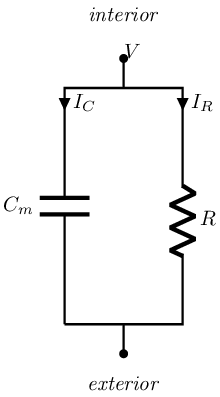
\includegraphics[scale=0.5]{../Figuras/bicapaLipidos.png}
 \caption{Modelo de la bicapa de lipidos donde, V son los cambios de voltaje en la membrana que es el potencial eléctrico,\(I_{C}\) es la corriente del capacitor, \(I_{R}\) es la corriente de la resistencia, \(C_{m}\) es la capacitancia de la membrana, R es la resistencia}
 \label{fig:circuitoP}
\end{figure}

Tenemos dadas las siguientes ecuaciones:
\begin{equation}
    I_{C} + I_{R} - I_{ext} = 0
  \label{eq:bicapa1}
\end{equation}

\begin{equation}
    C\dfrac{dV}{dt} + \dfrac{V}{R} - I_{ext} = 0 \\
  \label{eq:bicapa2}
\end{equation}

\begin{equation*}
    C\dfrac{dV}{dt} = -\dfrac{V}{R} + I_{ext} 
\end{equation*}

Ahora por la ley de corriente de Kirchhoff \footnote{La ley de la corriente de Kirchhoff dice que la suma de todas las corrientes que fluyen hacia un nodo es igual a la suma de las corrientes que salen del nodo} tenemos que la suma de las corrientes del capacitor y la recistencia debe ser cero
por la concervación de corriente y si consideramos un factor adicional de una corriente externa aplicada o administrada a la neurona, tenemos la ecuación \ref{eq:bicapa1}.

Después tenemos la relación entre la diferencia de potenciales, que almacena energía y la carga eléctrica que guarda, donde: \emph{C} es la capacidad, medida en faradios, \emph{Q} la carga eléctrica almacenada, medida en culombios, \emph{V} la diferencia de potencial medida en voltios. Entonces \(C = Q/V\), despejando a \emph{Q} tenemos \emph{Q = CV} y derivando de ambos lados respecto al tiempo y conciderando que \emph{C} es una constante al ser una propiedad de la membrana \(\dfrac{dQ}{dt} = C\dfrac{dV}{dt}\). Como la definición de corriente es el cambio de carga en el tiempo tenemos que \(I_{C} = C\dfrac{dV}{dt}\). Notemos finalmente la corriente de la resistencia \(I_{R}\), recordando la ley de Ohm \footnote{La ley de Ohm establece que la diferencia de potencial V que aplicamos entre los extremos de un conductor determinado es directamente proporcional a la intensidad de la corriente I que circula por el conductor, es decir \(V = R * I\). Notemos también que \(V = V_{m} - V_{rest}\) } la podemos rescribir como \(\dfrac{V-V_{rest}}{R}\). Sustituyendo de lo anterior en la ecuación \ref{eq:bicapa1} se obtiene la siguiente ecuación:

\begin{equation}
 C\dfrac{dV}{dt} + \dfrac{V-V_{rest}}{R} - I_{ext} = 0
 \label{eq:bicapa3}
\end{equation}

\begin{equation*}
 C\dfrac{dV}{dt} = -\dfrac{V-V_{rest}}{R} + I_{ext} 
\end{equation*}

Ahora multiplicando todo por R:
\begin{equation}
 RC\dfrac{dV}{dt} = -V + (V_{rest} + RI_{ext}) 
 \label{eq:bicapa4}
\end{equation}

Denotando RC como la constante de tiempo \(\tau\) y tomando en cuenta que en cuanto se aplica la corriente va a empezar a cambiar el voltaje poco a poco hasta establecerse en un voltaje de equilibrio (ahí se va a quedar quieta). Entonces cuando el voltaje ya no está cambiando con el tiempo quiere decir que su derivada con respecto al tiempo es cero. Observemos que \(dV/dt = 0\) significaría que V es igual a infinito y que el voltaje en el estado estacionario cuando , \(dV/dt = 0\) depende del potencial de reposo y del producto entre la resistencia con la corriente externa suministrada, entonces tenemos que:

\begin{equation}
 V_{\infty} = V_{rest} + RI_{ext}
 \label{eq:bicapa5}
\end{equation}

Sustituyendo con \ref{eq:bicapa5} y la constante, en \ref{eq:bicapa4} tenemos que:
\begin{equation}
 \tau\dfrac{dV}{dt} = -V + V_{\infty}
 \label{eq:bicapa6}
\end{equation}

\subsection{Las conductancias ionicas}
Nuestro objetivo aquí es encontrar ecuaciones que describan las conductancias con precisión razonable y lo suficientemente simples para el cálculo teórico de \emph{el potencial de acción} y \emph{el período refractario}. 

Si tomamos las ecuaciones diferenciales anteriores notamos que las soluciones tienen este tipo de forma \ref{fig:graficaX}:

\begin{figure}[h]
 \centering
 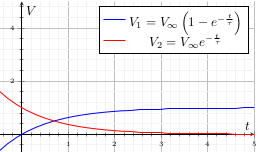
\includegraphics[scale=0.8]{../Figuras/solPulso1.png}
 \caption{Soluciones para el pulso.}
 \label{fig:graficaX}
\end{figure}


Donde si estamos aplicando una corriente externa lo que sucede es lo que estamos viendo en azul, un exponencial que va creciendo y que tiende hacia un cierto valor límite que sería de infinito. Si dejamos de aplicar la corriente externa entonces ahora tendremos un exponencial pero que tiende hacia el cero y se va a estabilizar en cero, lo que vemos en rojo. 

\begin{figure}[h]
 \centering
 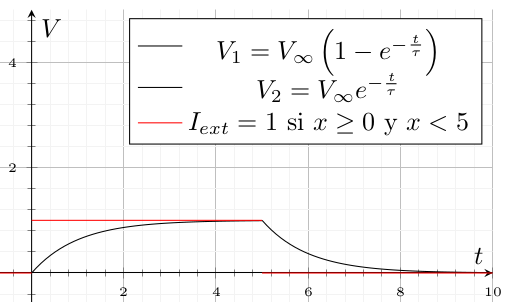
\includegraphics[scale=0.5]{../Figuras/solPulso2.png}
 \caption{Soluciones para el pulso escalón.}
 \label{fig:graficaX1}
\end{figure}

Simulando lo que hicieron Hodgkin y Huxley que fue al axón de repente darle un toque, siendo en el origen de la gráfica (que visualizamos en la figura \ref{fig:graficaX1}) la parte en la que le están dando el toque al axón, momentos antes estaba quieta la neurona de repente le aplican una cierta cantidad de electricidad y va a empezar a cambiar el comportamiento de los canales la porosidad de la membrana, vamos a ver que empieza a incrementarse la diferencia de potencial hasta que llegan a un nuevo equilibrio (alrededor de t = 3) y si siguieran dándole el toque en esa cantidad pues ya se quedaría ahí la neurona ya no veríamos más cambios lo que va a suceder entonces es que, retiramos las pinzas (se le deja de dar el toque) y los canales otra vez van a empezar a regresar a la normalidad y vamos a ver un descenso en adelante.

Entonces hasta aquí ya tenemos la idea de cómo va a reaccionar la neurona ante cierto estimulo, sin embargo esto que acabamos de ver en las gráficas sería como si tuviéramos un solo tipo de canal, ahora qué pasa si consideramos que tenemos diferentes tipos de canales pasando iones, en condiciones distintas. 
Aquí es donde va a importarnos el hecho de que existen diferentes tipos de canales con voltajes de equilibrio diferente. 
Retomando a los potenciales de Nerst \(E_{Na},E_{K},E_{L}\) notemos que están dados por:

\begin{equation}
    E = \dfrac{k_{B}T}{zq}\ln\dfrac{[adentro]}{[afuera]}
 \label{eq:diferenciaP}
\end{equation}

Estos potenciales están relacionados con las características termodinámicas, en la ecuación anterior \ref{eq:diferenciaP} \(k_{B}\) la constante de Boltzman, \(q\) es la carga del ion, y \(z\) es el número de iones. El logaritmo natural representando el promedio de cuántos elementos tenemos en la parte de adentro con respecto a cuántos elementos tenemos en la parte de afuera.

Considerando los diferentes puntos de equilibrio en los cuales se puede encontrar la diferencia de potencial en la membrana, vamos a distinguir entre tres estados de esta (también se puede ver en \ref{fig:graficaP}):

\begin{enumerate}
 \item \textbf{Polarizada} en su estado de reposo con \(V < 0 ( V \approx -70mV )\).
 \begin{itemize}
  \item Su estado de reposo,cuando la neurona no está haciendo nada simplemente están corriendo los sodios y entran los potasios.
 \end{itemize}
 \item \textbf{Despolarizada} cuando \(V \geq 0\).
 \begin{itemize}
  \item Cuando en sus dendritas y en el cuerpo de la neurona se acumula una carga muy grande, se abre la compuerta de sodio y van a empezar a entrar un montón de sodio, esta diferencia de potencial que existía entre lo fuera y lo adentro se va a reducir de hecho se puede llegar a reducir bastante dependiendo de la carga que le estemos aplicando.
  \item Valores positivos en la diferencia de potencial.    
 \end{itemize}
 \item \textbf{Hiperpolarizada} cuando la diferencia de potencial incrementa su magnitud \(V << 0\).
 \begin{itemize}
 \item En cuanto se despolarice van a empiezar unas interacciones  entre los diferentes tipos de canales que lo que van a intentar hacer es regresar a la neurona en su estado normal.
 \item Si antes estaba quieta a los -70mV aquí, ahora va a quedar todavía más abajo alrededor de -90mV. Esto va a permitir un fenómeno que se le conoce como \emph{el periodo de refracción} y ese periodo sirve para que simplemente se lance un disparo y que el comportamiento eléctrico no se rebote otra vez en dirección contraria en la neurona, va a quedar muy quieta la neuronas durante un rato y después regresará otra vez es su equilibrio. 
 \end{itemize}

\end{enumerate}
 
\section{Modelo de las compuertas iónicas controladas por voltaje}

Retomando el modelo del circuito electrico modelando la membrana, junto con los canales y los iones, volvamos a verlo ahora en la \ref{fig:circuito1}

\begin{figure}[H]
 \centering
 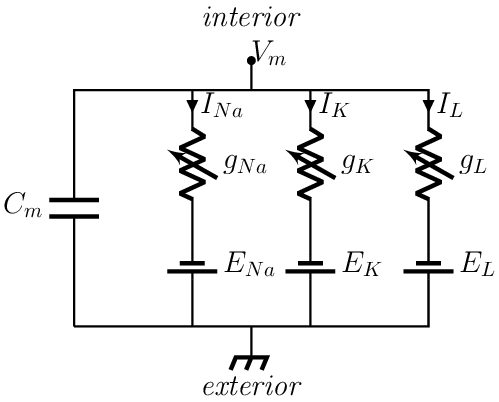
\includegraphics[scale=0.5]{../Figuras/circuito.png}
 \caption{Modelo de la membrana axónica modelada como circuito eléctrico, con los distintos canales presentes y su voltaje de reposo.}
 \label{fig:circuito1}
\end{figure}

Recordemos brevemente las definiciones de los dos tipos de canales protagonistas en el modelo:

\begin{definition}
 \emph{Canal persistente} Tiene un sólo tipo de compuerta y dos estados posibles:
 \begin{enumerate}
  \item \textbf{Activado}
  \item \textbf{Desactivado}
 \end{enumerate}

\end{definition}

\begin{definition}
 \emph{Canal transitorio} Tiene compuertas de activación e inactivación, y tres estados:
 \begin{enumerate}
  \item \textbf{Activado} Ambas compuertas abiertas.
  \item \textbf{Desactivado} Compuerta de activación cerrada, inactivación abierta.
  \item \textbf{Inactivada} Compuerta de inactivación cerrada.
 \end{enumerate}

\end{definition}


Y retomando \hyperlink{LaEq}{la primera ecuación diferencial} donde tenemos por un lado la corriente que está pasando a través del capacitor y por otro lado vamos a tener las corrientes que están circulando a través de los diferentes canales, 

\begin{equation}
  C_{m} \dfrac{dV_{m}}{dt} =  - g_{Na} m^3 h(V_{m} - E_{Na} ) - g_{K} n 4 (V_{m} - E_{K} ) - g_{L} (V_{m} - E_{L} ) + I_ext
  \label{eq:corrientesRepaso}
\end{equation}

Las capacitancias y variables del lado izquierdo estan explicadas en la sección \hyperlink{secc}{\emph{Modelo de la membrana como bicapa de lípidos}}, aqui vamos a retomar las ecuaciones \ref{eq:corrientesEnLaMembrana3},\ref{eq:corrientesEnLaMembrana4},\ref{eq:corrientesEnLaMembrana5} de esa misma sección, (recordemos que estás ecuaciones describen la probabilidad de que los canales ionicos esten abiertos) que son las siguientes:
\begin{equation}
  \dfrac{1}{\gamma(T)}\dfrac{dn}{dt} =  \alpha_{n^\infty} (V)(1 - n) - \beta_{n} (V) n = \dfrac{n(V)-n(t)}{\tau_{n}(V)}
  \label{eq:probabilidades1}
\end{equation}

\begin{equation}
  \dfrac{1}{\gamma(T)}\dfrac{dm}{dt} =  \alpha_{m} (V)(1 - m) - \beta_{m} (V) m = \dfrac{m^\infty(V)-m(t)}{\tau_{m}(V)}
  \label{eq:probabilidades2}
\end{equation}

\begin{equation}
  \dfrac{1}{\gamma(T)}\dfrac{dh}{dt} =  \alpha_{h} (V)(1 - h) - \beta_{h} (V) h = \dfrac{h^\infty(V)-h(t)}{\tau_{h}(V)}
  \label{eq:probabilidades3}
\end{equation}

Ahora notemos los elementos en estás ecuaciones anteriores con \(ion\) pudiendo denotar las compuertas del potasio \(n\) o del sodio, ya sea \(m\) o \(h\):
\begin{itemize}
 \item \(\dfrac{1}{\gamma(T)}\) Este es el coeficiente de escala temporal, dependiente de la temperatura los por eso está apareciendo aquí una \(t\). Para las simulaciones que nosotros vamos a hacer vamos a pensar que estamos en una temperatura fija. 
 \item \(\alpha_{ion}(V)\) probabilidad de que una compuerta transite de abierta a cerrada.
 \item \(\beta_{ion}(V)\) probabilidad de que una compuerta transite de abierta a cerrada.
 \item \(ion^\infty(V)\) probabilidad de compuerta abierta en el equilibrio cuando \(t \rightarrow \infty\) .
 \item \((ion)\) Probabilidad de que cada compuerta (n,m,h) esté abierta.
 \item \((1-ion)\) Probabilidad de que cada compuerta (n,m,h) esté cerrada.
 
 \item \(\tau_{ion}(V)\) Tiempo que toma llegar al equilibrio.
\end{itemize}


Lo que vamos a ver es que forma de escribir la ecuación depende precisamente del número de compuertas que tenían para poder abrirse y cerrarse. Reescribir la ecuación de esta manera lo que nos permite es medirlo en términos de estas probabilidades de que se abran y cierren las compuertas que serían 

Esta probabilidad se empieza a alterar conforme cambiamos el voltaje pero no va a llegar a su valor de equilibrio sino hasta después de pasado un cierto periodo.


\section{Dinámica del voltaje durante un disparo} 
\begin{figure}[H]
 \centering
 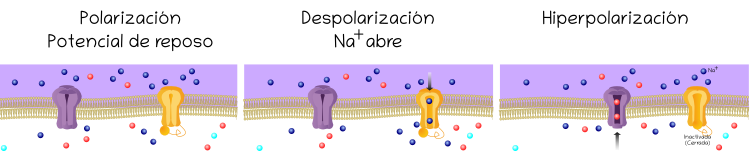
\includegraphics[scale=0.5]{../Figuras/polarizacion1.png}
 \caption{Dinámica del voltaje.}
 \label{fig:voltaje1}
\end{figure}

\begin{figure}[H]
 \centering
 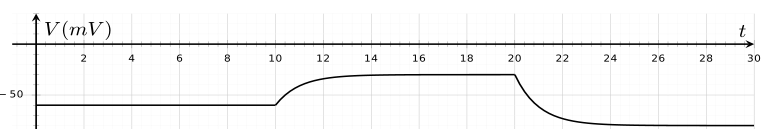
\includegraphics[scale=0.5]{../Figuras/polarizacion2.png}
 \caption{Pulso, cuando se rebasa el voltaje umbral, los canales de Na + y K + interactúan para producir
una rápida despolarización de la membrana, para luego hiperpolarizarla}
 \label{fig:voltaje1}
\end{figure}

\begin{figure}[H]
 \centering
 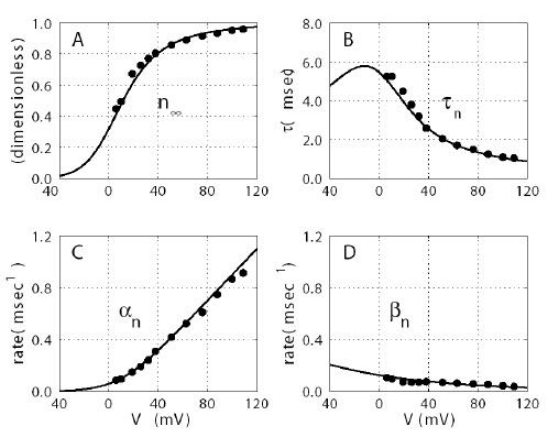
\includegraphics[scale=0.5]{../Figuras/medidasExperimentales.png}
 \caption{Medición experimental de los parámetros y ajuste manual de curvas. Imagen de Nelson
2004}
 \label{fig:voltajeAB}
\end{figure}

\begin{figure}[H]
 \centering
 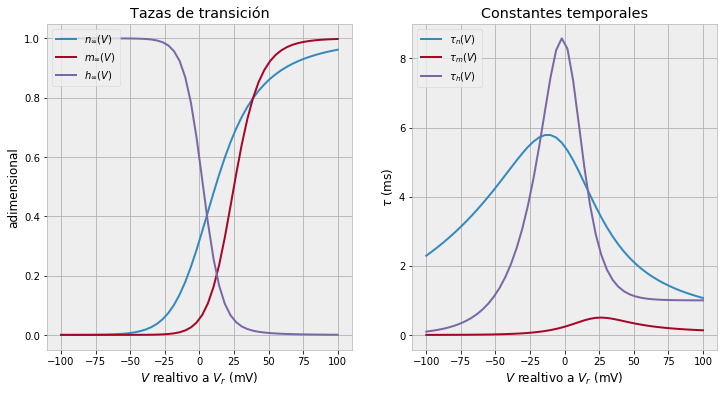
\includegraphics[scale=0.5]{../Figuras/actinac.png}
 \caption{Las compuertas de Na + se abren primero, luego las de K + y esto provoca que se inactiven las de Na + .}
 \label{fig:voltajeActInac}
\end{figure}

\begin{figure}[H]
 \centering
 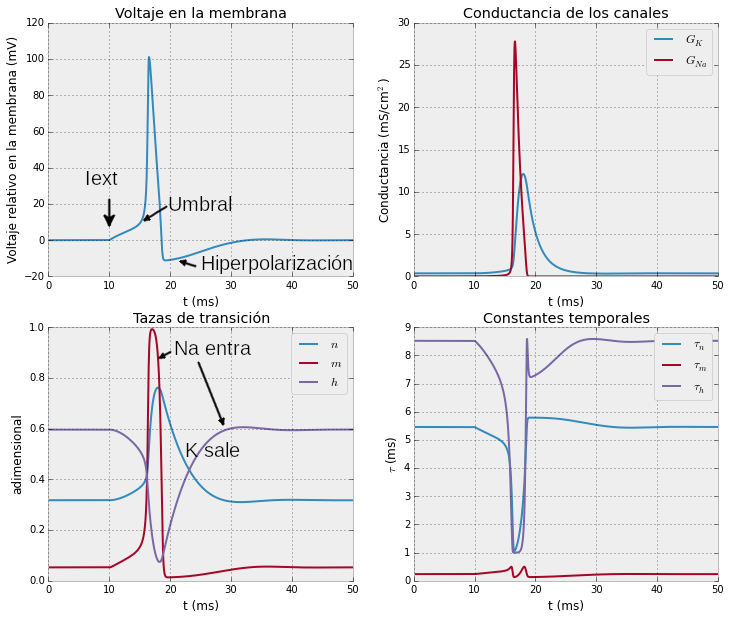
\includegraphics[scale=0.5]{../Figuras/disparo.png}
 \caption{Medidas experimentales de los estimulos y la reacción de los canales}
 \label{fig:voltajeActInac}
\end{figure}


\section{Simulación usando el método de Euler}
debemos alistarse rápidamente como estamos resolviendo esas ecuaciones diferenciales ya para tener una simulación numérica y se trata del algoritmo de integración de hoy no vamos a tener una solución explícita en nuestro sistema de ecuaciones sino que vamos a utilizar esta técnica en la que comenzamos con un valor inicial y a partir de ahí utilizamos las ecuaciones para calcular las tangentes aproximamos a la curva con su tangente y vamos avanzando paso a pasito entonces para ver cómo se comportan entonces estas gráficas que vamos a ver en la parte de arriba se obtuvieran precisamente con el método de boiler y ahorita le vamos a llamar la función integra disparo necesitamos cuatro valores que van a ir este que van a provocar diferentes comportamientos el primero es durante cuánto tiempo queremos correr la simulación el segundo que tan finos queremos que sean los pasos recordemos que vamos a aproximar la función con segmentos de recta siguiendo la tangente entonces si estos pasos son demasiado grandes y la curva ya se separó mucho del superagente entonces nuestra simulación va a ser mala y la función que obtengamos no se va a parece mucho la solución si hacemos pasos demasiado pequeños nos vamos a tardar demasiado en hacer el cómputo entonces hay que encontrar aquí un buen equilibrio entre ambos casos lo siguiente que vamos a necesitar es el voltaje inicial en donde empieza nuestra simulación donde estaba en nuestra neurona cuando empezamos a trabajar y el siguiente dato que necesitamos es la corriente externa de qué magnitud fue el toque que le estamos dando en este momento al action con estos datos entonces ya podemos ir calculando todos los demás elementos aquí ya no quise mencionar las constantes como las que me dieron joaquín y huxley precisamente porque son constantes entonces les pueden definir en cualquier lugar como parámetros fijos el siguiente paso bueno vamos a querer guardar lo que está ocurriendo para todos los tiempos desde cero hasta t en cada delta te lo estoy mencionando aquí como una serie de arreglos donde en la posición 0 viene nuestra primera medición en la posición 1 nuestra siguiente aproximación etcétera etcétera vamos a tener toda una serie de puntos donde estamos guardando estos pasos para inicializar oyler sabemos que necesitamos es un primer valor a partir del cual vamos a calcular la tangente y vamos a ir aproximando lo demás entonces para eso queríamos el voltaje inicial como nosotros sabemos donde estaba en reposo nuestra célula originalmente vamos a poder guardar ese voltaje como el primer valor para nuestra simulación ahora todos los demás elementos las alfa las betas etcétera etcétera se pueden calcular si ya conocíamos ese voltaje inicial entonces a partir de este momento podemos repetir el mismo ciclo tantas veces como sea necesario para cubrir el intervalo desde el tiempo inicial hasta el tiempo t brincando del rate en del tati entonces dado un voltaje vamos a calcular las diferentes alfaz que son las que se medían experimentalmente originalmente utilizando las ecuaciones que encontraron joaquín y jujuy a partir de estas el fasi estas vetas entonces ahora si podemos calcular las nm h todas las dos que son las que estamos usando acá ya teniendo estas entonces podemos calcular las probabilidades para las compuertas nm h utilizando las ecuaciones en diferencias en forma matricial ahora aquí esta parte fue importante sobre todo por el asunto de las pérdidas numéricas es recordemos que la computadora tiene una representación en punto flotante lo cual quiere decir que un número real no se puede representar en la computadora voy a pasar a la siguiente cuando lleguemos al cálculo de las generadas las secas y lleguemos finalmente a calcular el voltaje b nos va a importar exactamente como escribimos los términos por el problema del truncamiento a qué me refiero supongamos que tenemos un número real este número no lo podemos representar en la computadora en algún momento se nos acaba el espacio y vamos a tener que volar nos todos los dígitos que hubieran seguido acá concretamente se va a notar eso mucho aquí en la simulación del modelo de hodgkin y hawkes y entonces cada vez que nosotros tocamos estos dígitos estamos perdiendo precisión si nosotros por ejemplo en vez de dividir 3.14 16 entre 2.25 hacemos esto 35 en una computadora vamos a obtener este resultados diferentes por eso que les dimos si les estamos diciendo cuando separar cuando no separar para que todos podamos obtener los mismos resultados desde más ojo con esa parte porque a veces puede ser que no les salgan los disparos pero porque primero dicen ha de sumar lo que será la división o primero la división y luego era de suma y estaba había que calculando en el orden diferente y es por eso les estamos poniendo aquí paso por paso cómo le tenemos que hacer en qué orden para hacer los cálculos es bueno una vez que ya terminamos de calcular estos términos que se van a necesitar en la ecuación más grande que es la del voltaje de la membrana podemos ir almacenando en los resultados temporales dentro de nuestros arreglos en la casilla que les corresponda para ese paso y aquí es donde ya vamos a utilizar la corriente externa para meterla en la ecuación diferencial para el voltaje una vez que tengamos esto tenemos que repetirlo para cada paso los observen que esto es como que para el tiempo t se calcula entonces estas y esa onda va a dar el siguiente valor del voltaje ya teniendo el siguiente valor del voltaje lo voy a poder utilizar para el siguiente paso y así nos vamos a seguir todo el tiempo si devolvemos estos bueno después ya nos vamos a poder permitir graficar qué fue lo que sucedió con cada uno de ellos y eso es precisamente de dónde sale esta imagen que tenemos aquí y todo lo referente a la simulación numérica.

\section{Información condificada en las dendritas}



\chapter{Aprendizaje de máquina}
\section{Espacio de hipótesis}
\section{Conjuntos de entrenaiento, validación y prueba}
\section{Perceptrón}
\section{Compuertas lógicas con neuronas}
\section{Funciones de activación}
\section{Funciones de error: diferencias al cuadrado y entropía cruzada}
\section{Medidas de rendimiento:}
\subsection{Matriz de confusión}
\subsection{Precisión}
\subsection{Recall}
\subsection{f score}

\part{Redes dirigidas acíclicas}
\chapter{Perceptrón multicapa}
\section{XOR}
\section{Propagación hacia adelante manual}
\section{Propagación hacia adelante vectorizada (con matrices)}
\section{Interpretación matemática del mapeo no lineal}
\section{Propagación hacia adelante para el perceptrón multicapa}


%%
\chapter{Entrenamiento por retropropagación}
\section{Función de error}
\section{Gradiente de la función de error}
\section{Descenso por el gradiente}
\section{Otros algoritmos de optimización}

\chapter{Optimización del entrenamiento} 
\section{Problemas en redes profundas}
\section{Gradiente desvaneciente (o que explota) }
\section{Entrenamiento en línea vs en lotes}
\section{Normalización y normalización por lotes}
\section{Regularización}

\chapter{Caso de análisis e interpretación}

\section{Red Hinton árbol familiar con numpy (entrenamiento)}

\section{Red Hinton árbol familiar con pytorch}

\chapter{Entrenamiento con genéticos}
%\section{MNIST versión básica con numpy}
\section{Algoritmos genéticos}
\section{Neuroevolución}
\subsection{Antecedentes: Aprendizaje por refuerzo en videojuegos}
\subsection{Arquitectura para estimar la función de recompensa}
\subsection{Entrenamiento}

%\part{Aprendizaje no supervisado}
\chapter{Mapeos autoorganizados}
\section{Aprendizaje no supervisado}
\section{Mapeos autoo-organizados}
\section{Kohonen}

%%
%\part{NO TIENE NOMBRE}
\chapter{Redes Neuronales Convolucionales}
\section{Convolución}
\section{Redes Convolucionales}
\section{Softmax}
\section{MNIST}

%%
\part{Redes con ciclos}
\chapter{Redes Neuronales Recurrentes}
\section{Derivadas ordenadas}
\section{Retropropagación en el tiempo}
\section{Sistemas dinámicos y despliegue del grafo}
\section{Arquitectura recurrente universal}
\section{Función de error}
\section{Forzamiento del profesor}

\chapter{Atención}
%\section{Casos de análisis de serie}
\chapter{LSTM}
\chapter{GRU}
\chapter{Casos de análisis: etiquetado de palabras y conjugación de verbos}

\part{Redes no dirigidas}
\chapter{Redes de hopfield}
\section{Entrenamiento}

\chapter{Máquinas de Boltzman}
\section{Entrenamiento}
\subsection{Partículas y partículas de fantasía}
\subsection{Máquinas de Boltzman Restringidas}

\chapter{Redes adversarias}
\section{GANs}

\appendix 
\chapter{Ecuaciones diferenciales}

%----------------------------------------------------------------------------------------
% Bibliografia
%----------------------------------------------------------------------------------------
\backmatter

\printbibliography[heading=bibintoc]

\end{document}
